\documentclass[11pt]{article}
\usepackage[utf8]{inputenc}
\usepackage{amsmath}
\usepackage{amssymb}
\usepackage{amsthm}
\usepackage{fullpage}
\usepackage{setspace}
\usepackage{enumerate}
\usepackage{subcaption}
\usepackage{graphicx}
\usepackage{floatrow}
\usepackage{float}
\newfloatcommand{capbtabbox}{table}[][\FBwidth]

\title{A Game of Inches: the Sabermetric Impact of Raising the Strike Zone }
\author{Kyle Burris\footnote{Department of Statistical Science, Duke University, Durham, NC, 27705.  Email: kyle.burris@duke.edu}}
\date{February 20, 2017}

\begin{document}

\maketitle

\section{Background}
On February 6, 2017, the MLB presented two new rule changes for the players' union to consider, according to ESPN's Jayson Stark.  One of these rule changes would redefine the lower edge of the strike zone to be the top of the batter's knees, opposed to ``the hollow beneath the kneecap."  This redefinition would raise the bottom half of the strike zone by an estimated two inches, theoretically boosting offensive output.\\

In a zero-sum league, teams do not have the luxury of waiting until games are played with the new strike zone to change their decision making.  To gain a competitive advantage, teams need to begin forecasting the impact of this rule now.  Raising the strike zone will benefit some players more than others.  Identifying these players will enable R\&D oriented teams to exploit market inefficiencies in the years immediately following implementation.\\

In this Hackathon analysis, I pose and attempt to answer the following questions: what will be the global MLB impact of raising the strike zone by two inches?  Which batters will benefit the most?  Which pitchers will suffer the most?  The work presented here is not meant to be all-encompassing, but rather a springboard from which to begin thinking about this problem.  Even if the rule is not implemented this coming season, the work will remain valid if and when the players' union eventually approves the change.

\section{The Evolution of the Strike Zone}
Although the formal definition of the strike zone has remained the same since 1996, umpire interpretation of the strike zone has changed a great deal in the past ten years.  With the increasing use of video technology in evaluating umpire decisions, umpires have been calling games more uniformly and in accordance with the letter of the rulebook.  In doing so, they have effectively expanded the lower edge of the strike zone.\\

To illustrate this effect, I fit a thin-plate logistic regression spline for pitches taken in the 2008 and 2016 seasons, including variables such as location, pitch type, and batter handedness.  For a brief primer on splines, I refer the reader to the Appendix.  Figure 1 displays the estimated probability of a called strike for a four-seam fastball delivered to a 6'2" right-handed hitter in both 2008 and 2016.  Note the expansion of the bottom of the strike zone in 2016.  The overlaid white strike zone represents the strike zone coordinates defined by Mike Fast in 2011.

\begin{figure}[ht]
\centering
\begin{subfigure}[b]{0.48\textwidth}
\centering
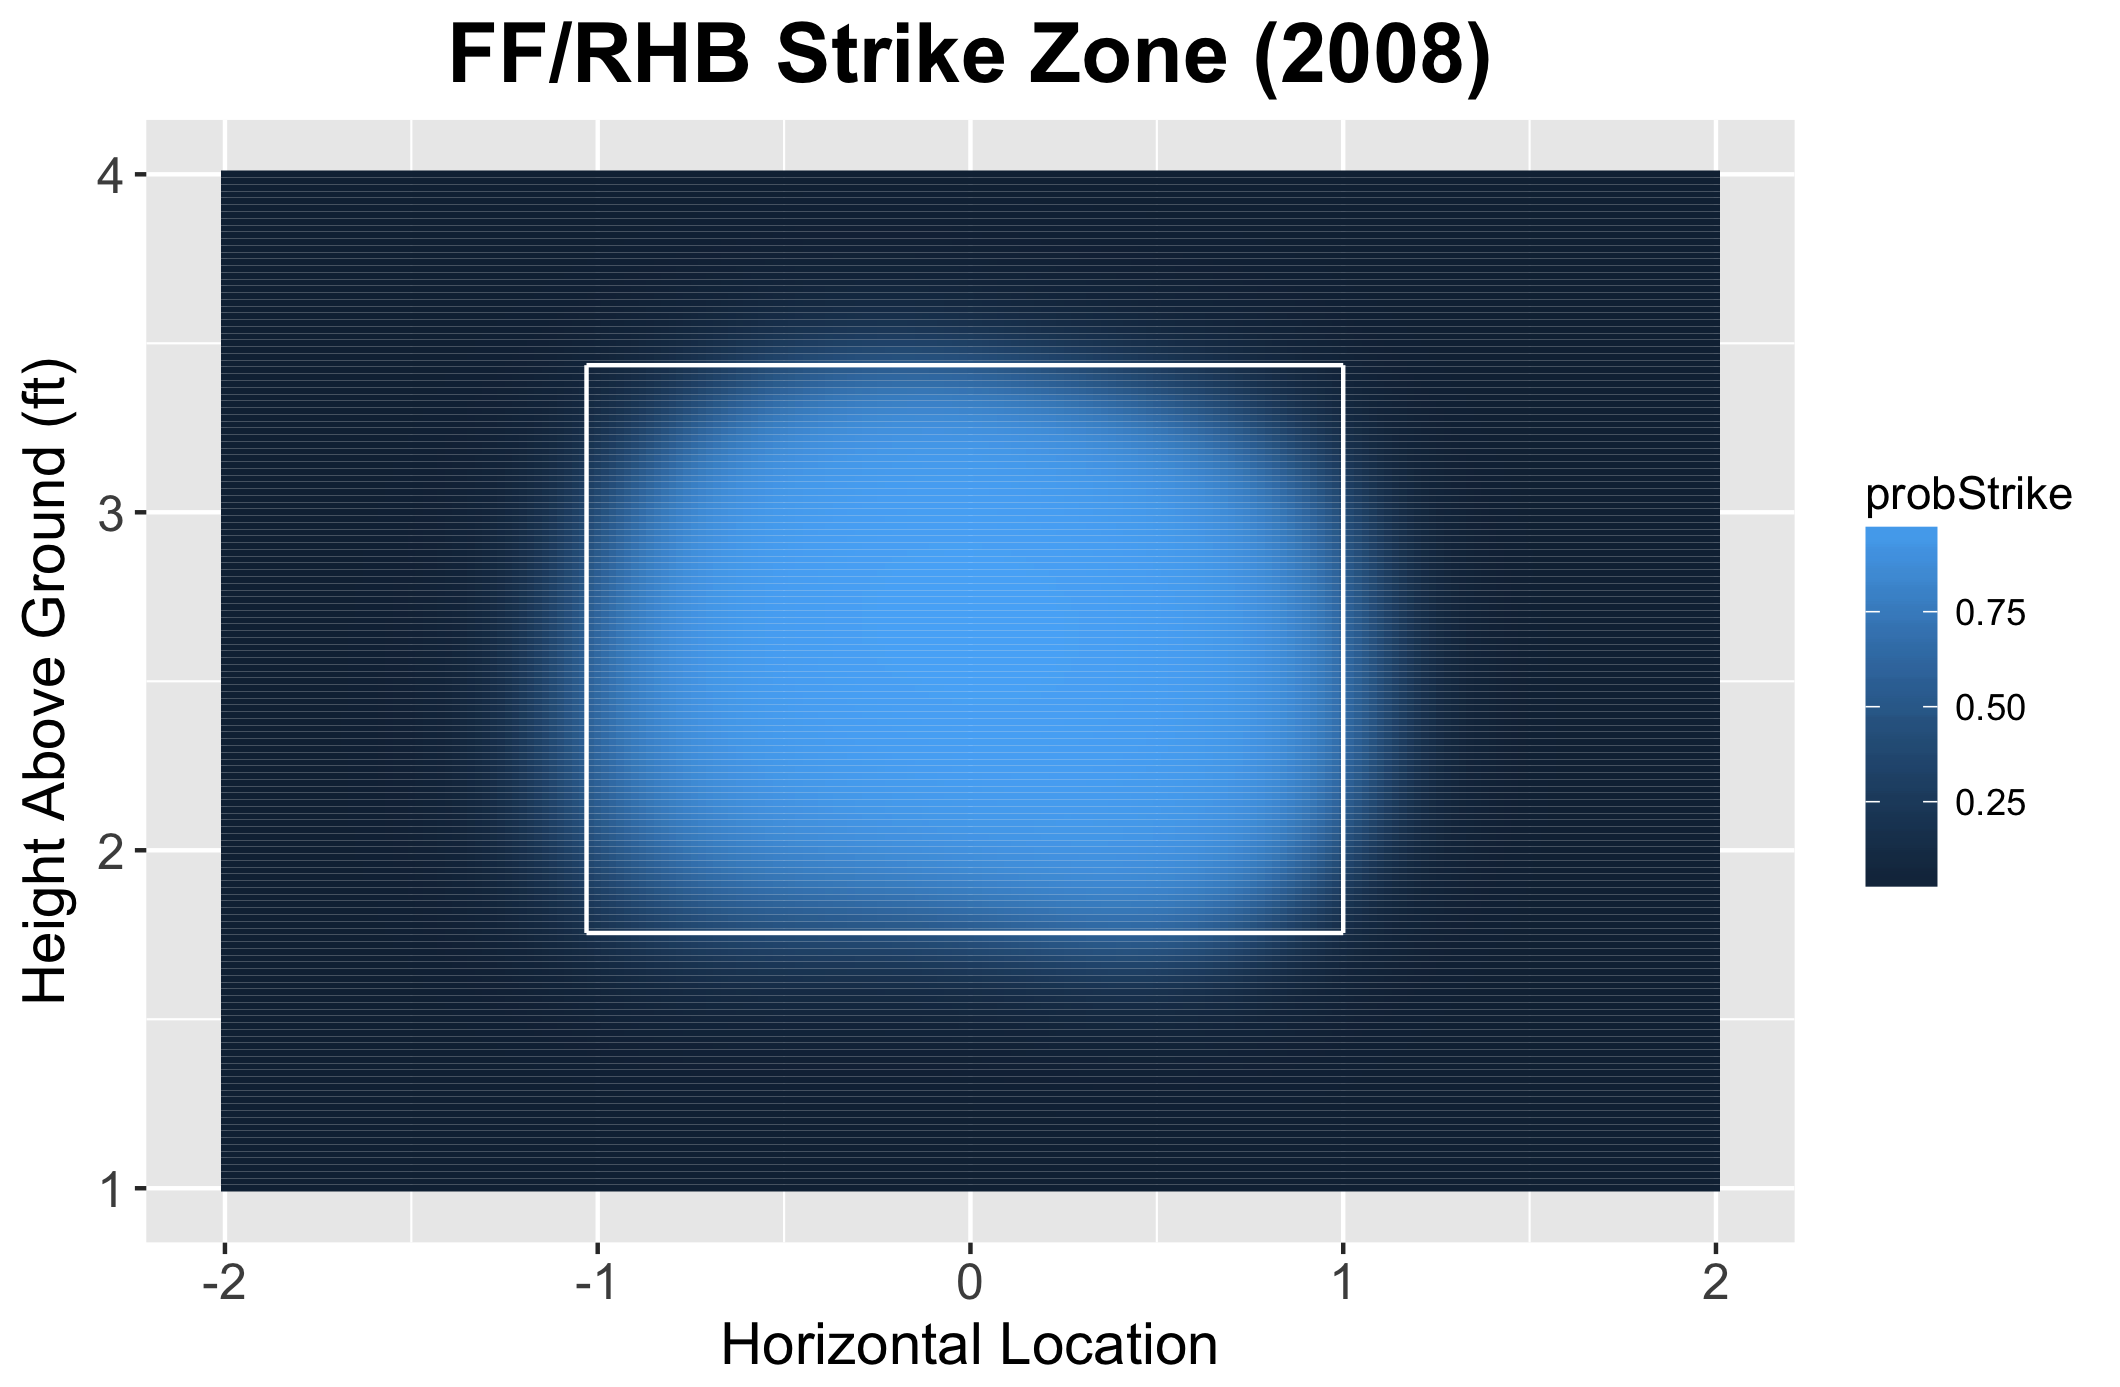
\includegraphics[height = 5.2cm]{../Output/fig1a.png}
\end{subfigure}
\begin{subfigure}[b]{0.48\textwidth}
\centering
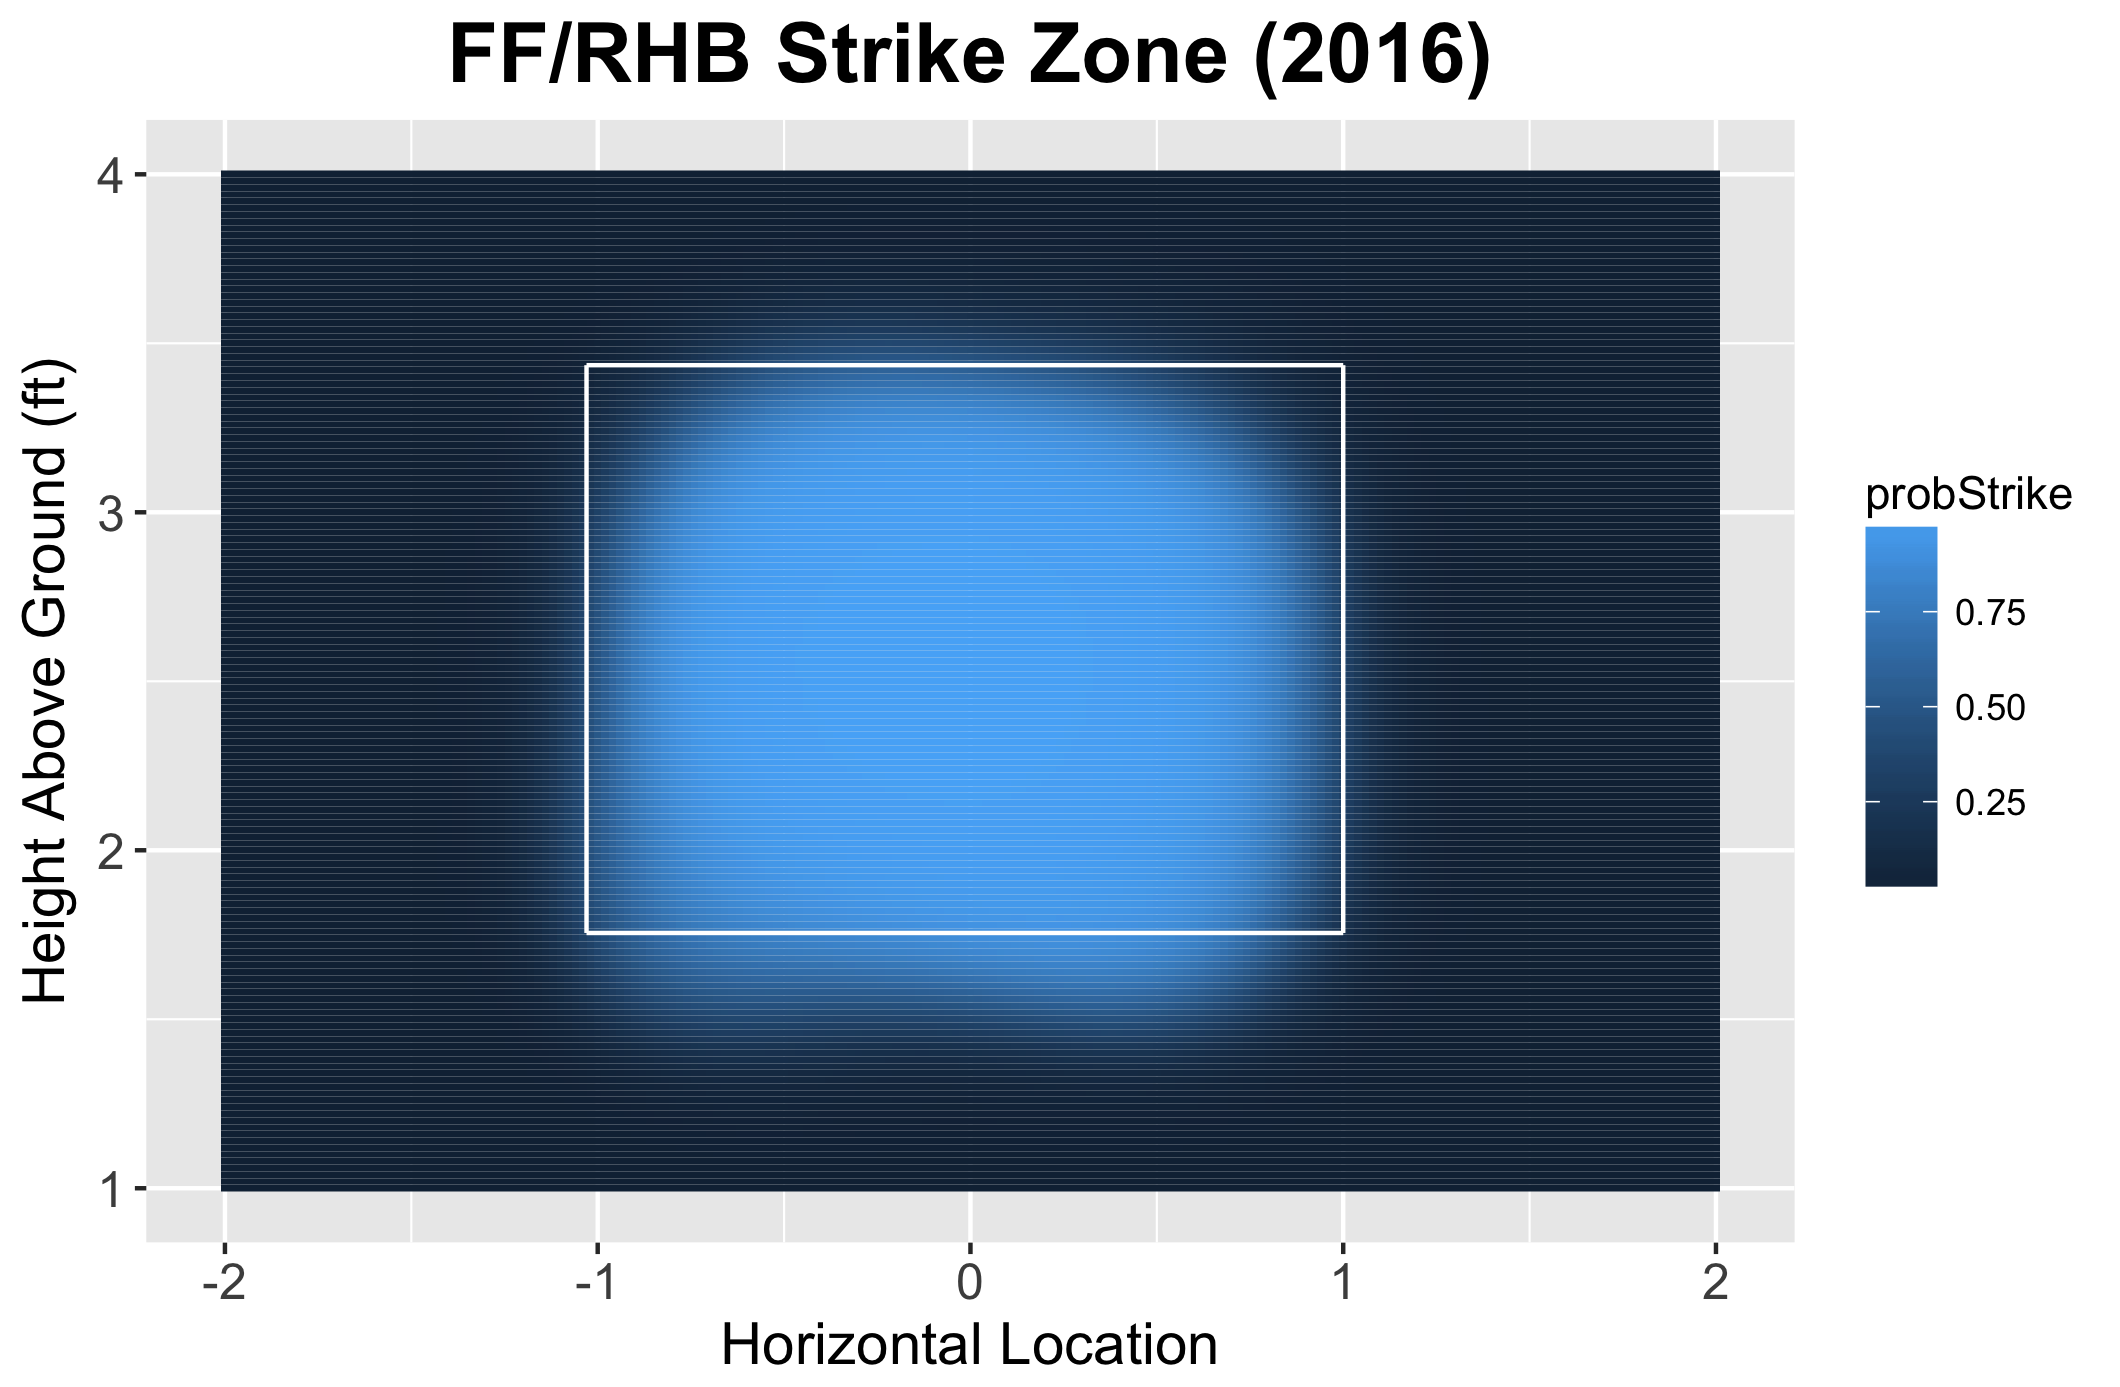
\includegraphics[height = 5.2cm]{../Output/fig1b.png}
\end{subfigure}
\caption{The Downward Expansion of the Strike Zone}
\end{figure}

When did this change occur?  How far has the strike zone dropped?  I define the \textit{empirical lower edge} (ELE) of the strike zone as the following: the estimated minimum vertical location at which an umpire is indifferent between calling a four-seam fastball that crosses the middle of the plate a ball or a strike.  I estimate this value by fitting a factor spline for all four-seam fastballs crossing the heart of the plate and finding the vertical location at which the estimated probability of a called strike is 0.5.  Table 1 and Figure 2 illustrate how the empirical lower edge of the strike zone has changed between 2008 to 2016.


\begin{figure}[ht]
\begin{floatrow}
  \capbtabbox{
\begin{tabular}{cccc}
  \hline
Year & ELE (ft) & Change & Difference \\ 
  \hline
2008 & 1.714 &  -& 0.176 \\ 
  2009 & 1.703 & -0.011 & 0.165 \\ 
  2010 & 1.683 & -0.020 & 0.145 \\ 
  2011 & 1.662 & -0.021 & 0.124 \\ 
  2012 & 1.608 & -0.054 & 0.070 \\ 
  2013 & 1.580 & -0.028 & 0.042 \\ 
  2014 & 1.544 & -0.036 & 0.006 \\ 
  2015 & 1.518 & -0.026 & -0.020 \\ 
  2016 & 1.538 & 0.020 & 0.000 \\ 
   \hline
   \caption{ELE Values by Year}
\end{tabular}
} 


\ffigbox{%
  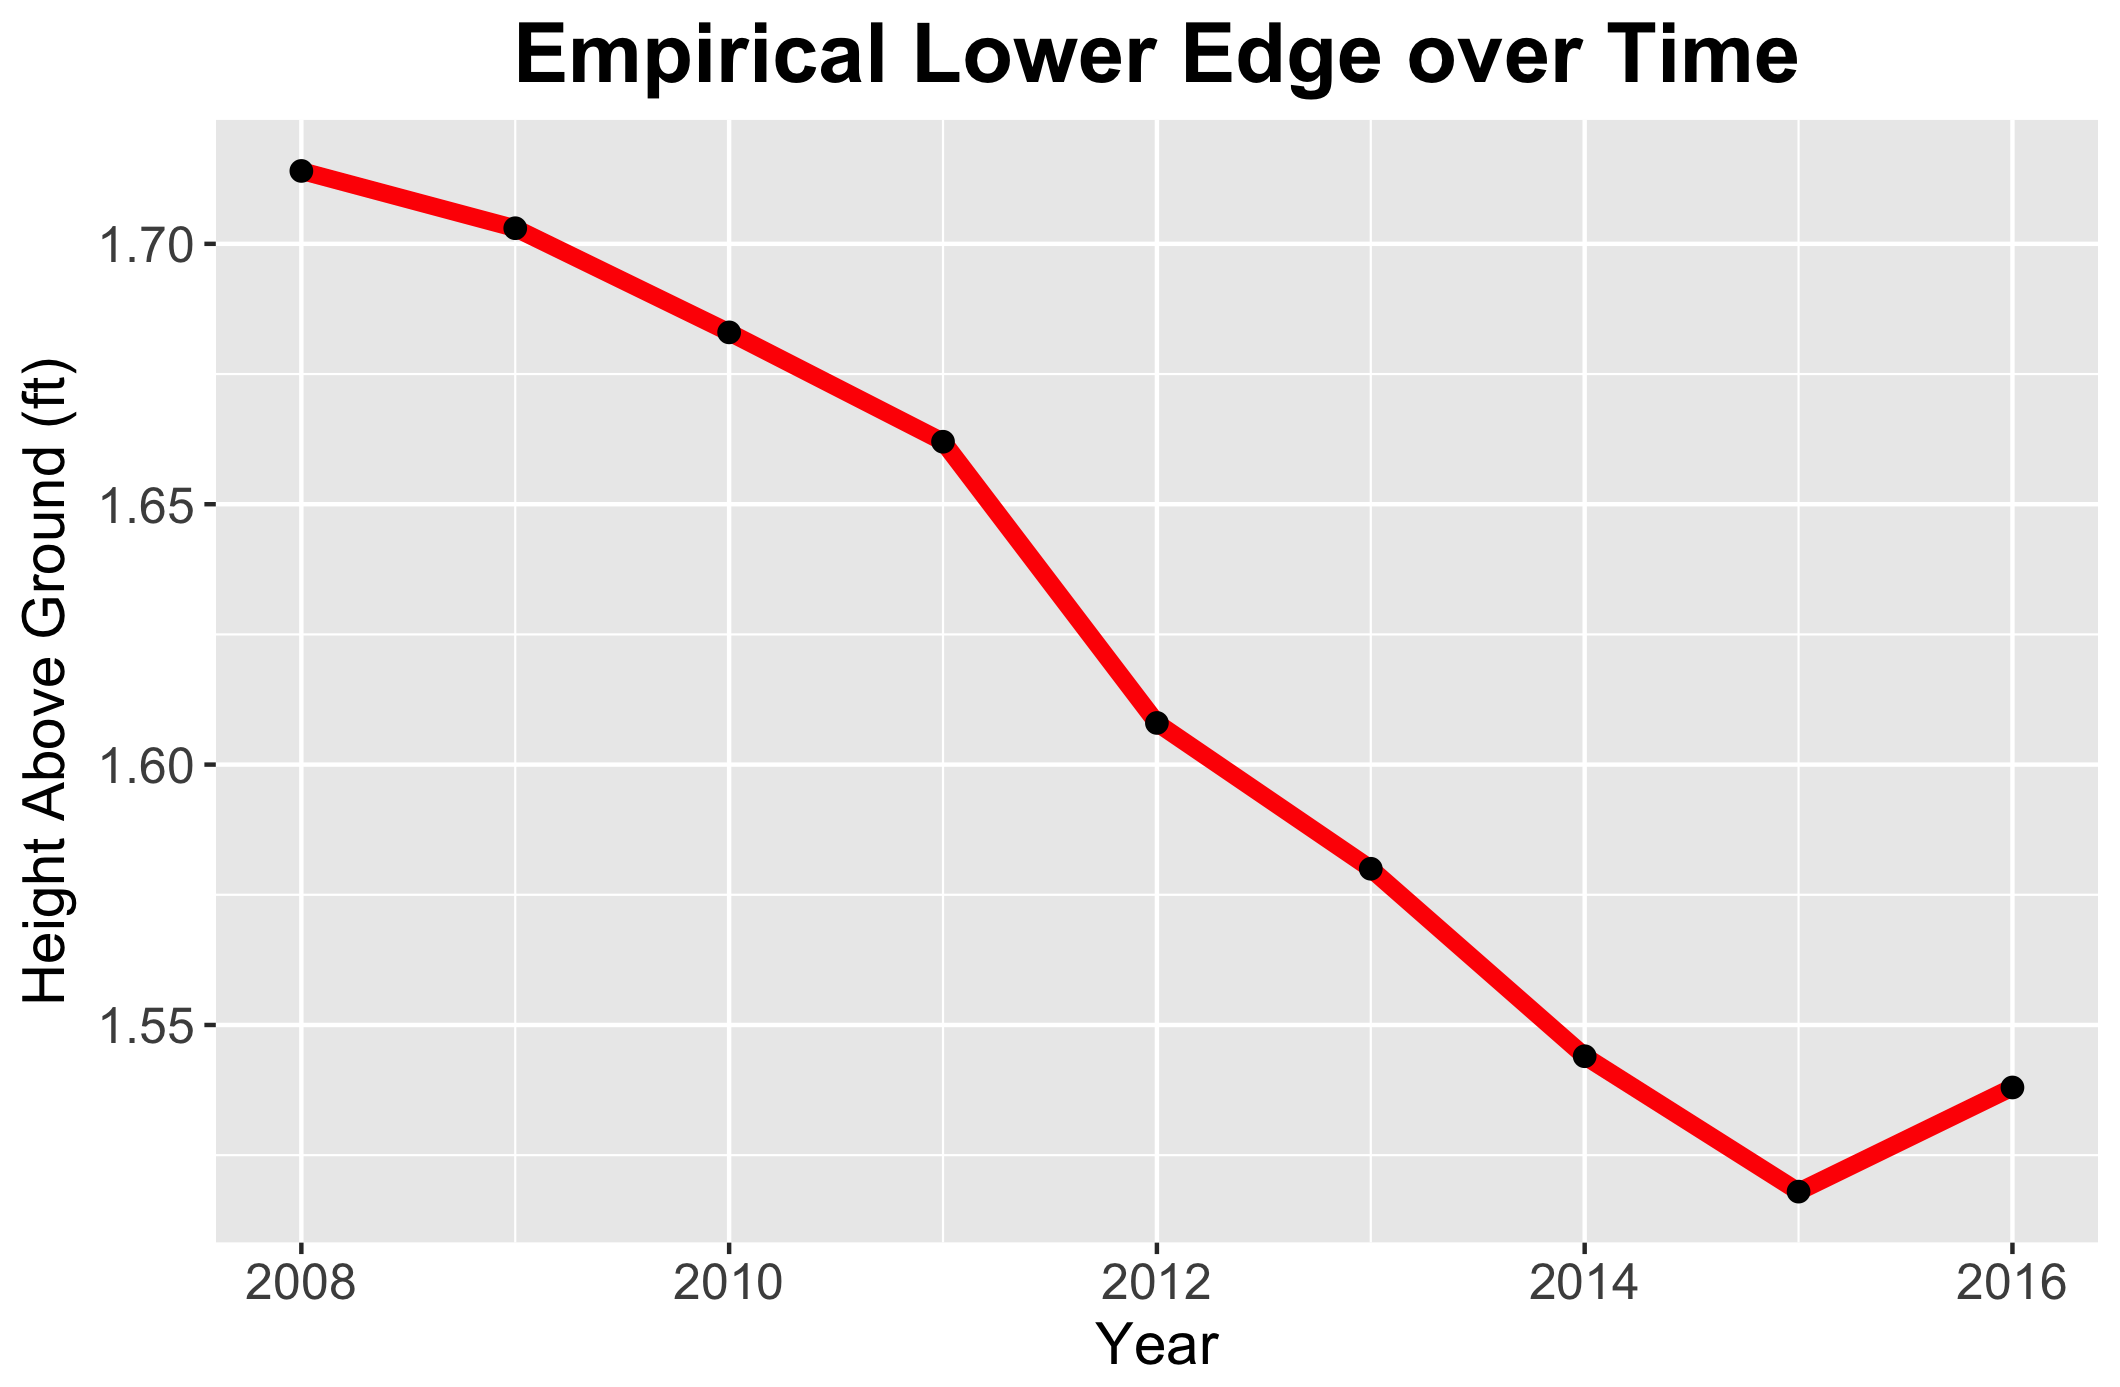
\includegraphics[width=.45\textwidth]{../Output/fig2b.png}%
}{%
\caption{ELE Over Time}
}

\end{floatrow}

\end{figure}
  
As you can see, the lower edge of the strike zone steadily decreased at a rate of roughly a quarter of an inch per year until 2015, when it began to level off.  Between 2008 and 2016, the lower edge of the strike zone dipped by 0.176 feet, or a little over two inches.  Because the new rule will raise the lower edge of the strike zone by an estimated two inches, this is a huge result for us.  In essence, we've already seen hundreds of thousands of pitches thrown under the new strike zone; they were thrown a little under ten years ago!  

\section{Global MLB Impacts}
Therefore, the new rule will essentially reverse the adjustments made by the batters and pitchers in response to the strike zone expansion between 2008 and 2016.  In conjunction with analysis suggesting that batters struggle hitting low pitches, pitchers began exploiting this rule by pounding the lower edge of the strike zone with impunity.  Figure 3 illustrates how the distribution of fastballs and curveball locations changed between 2008 and 2016.

\begin{figure}[ht]
\centering
\begin{subfigure}[b]{0.48\textwidth}
\centering
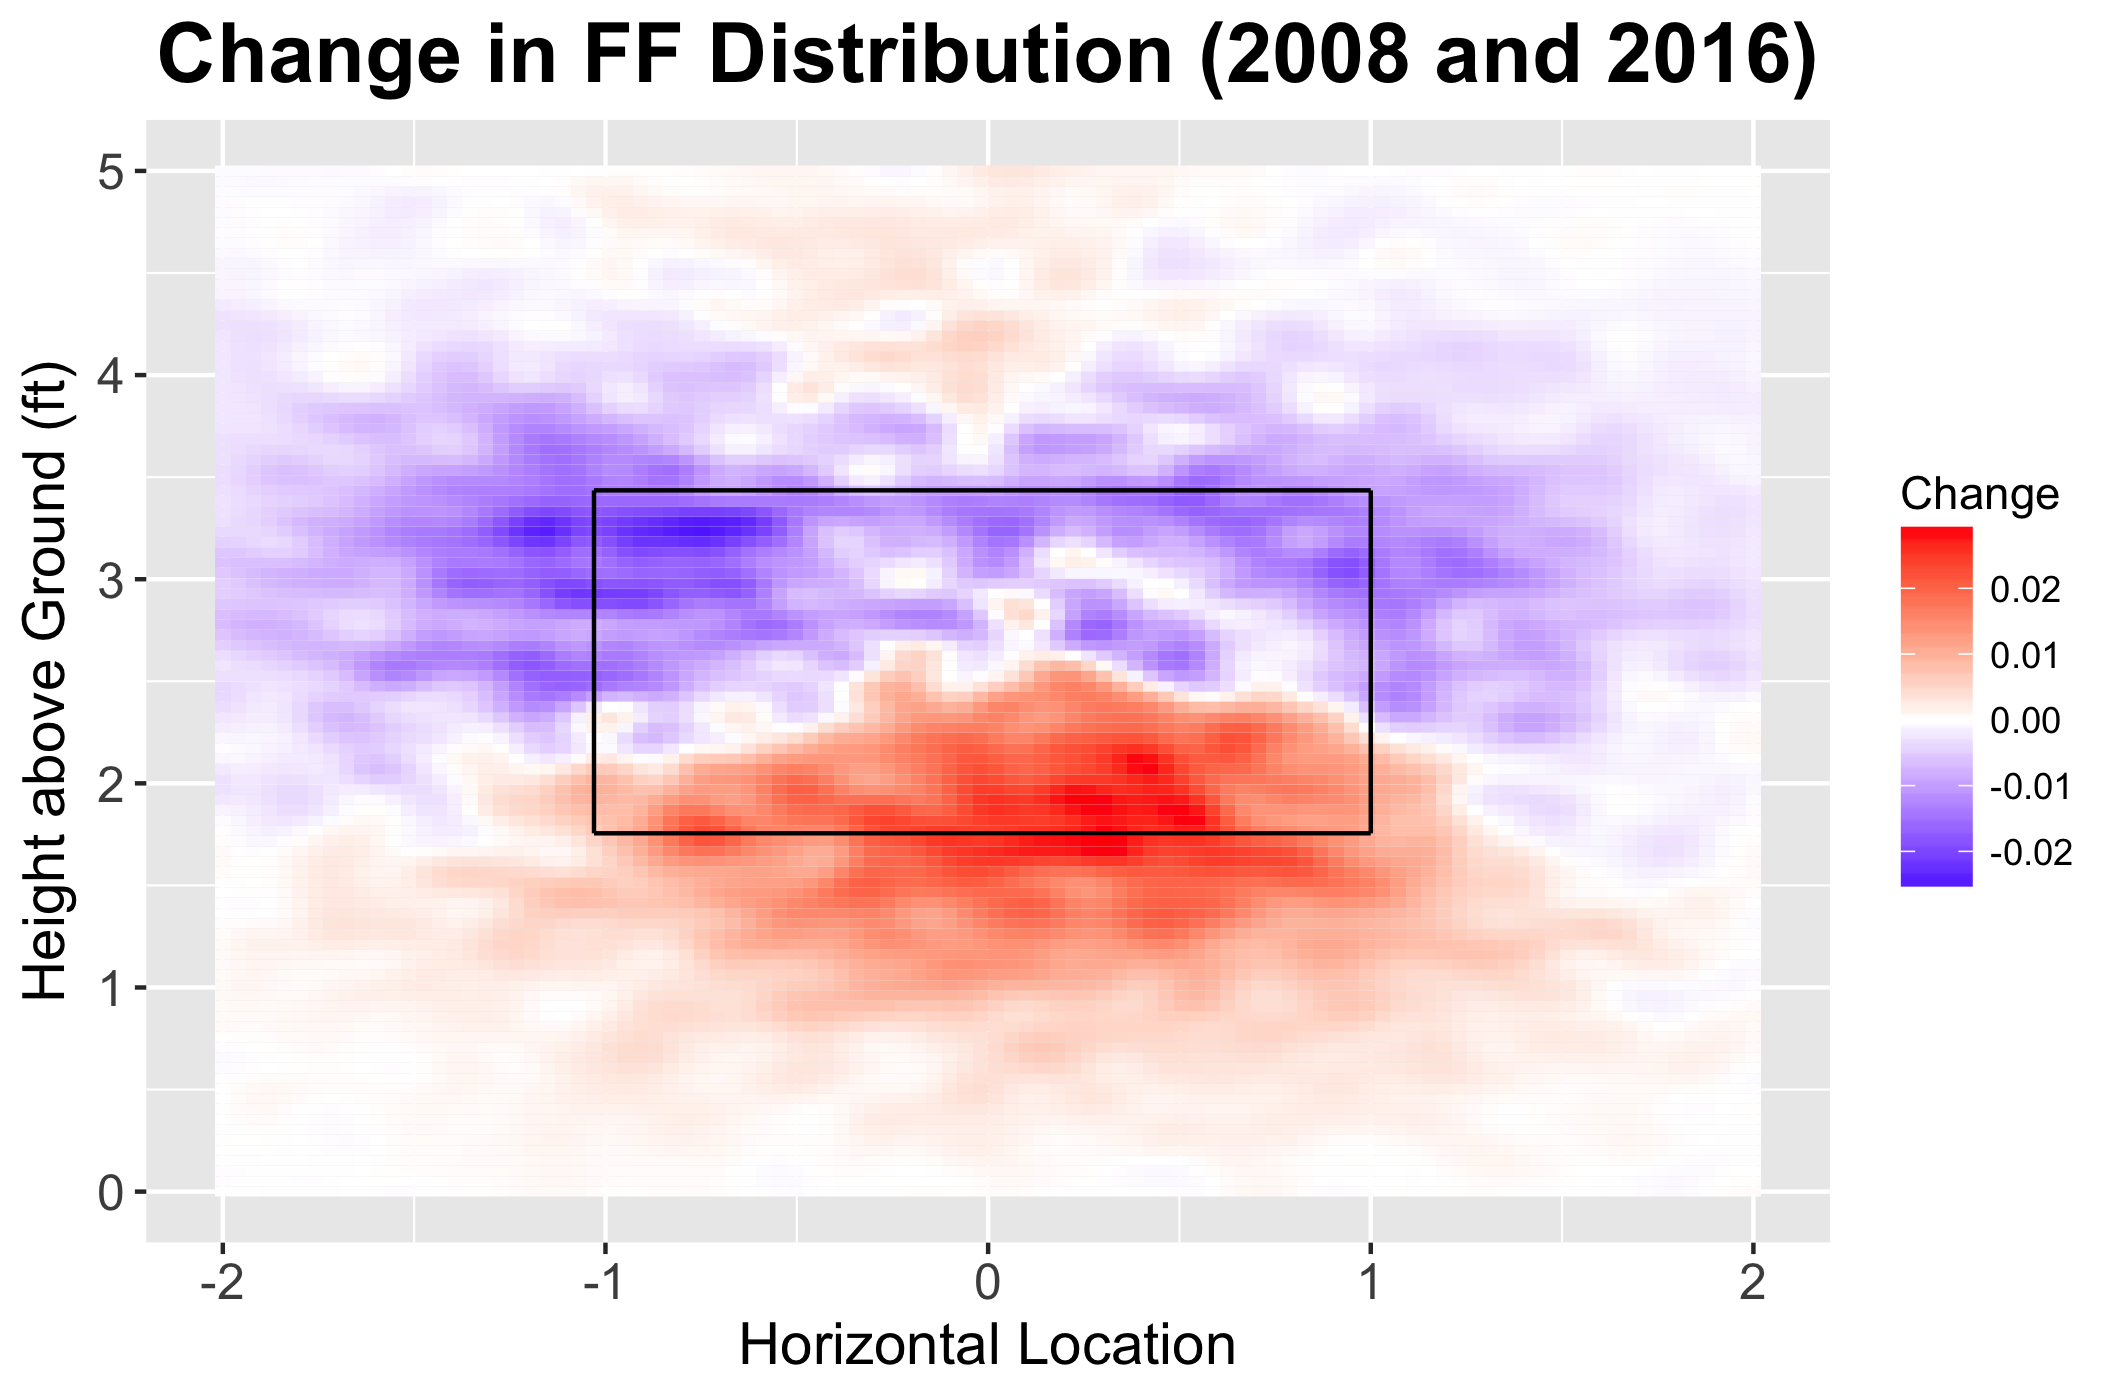
\includegraphics[height = 5.2cm]{../Output/fig3a.png}
\end{subfigure}
\begin{subfigure}[b]{0.48\textwidth}
\centering
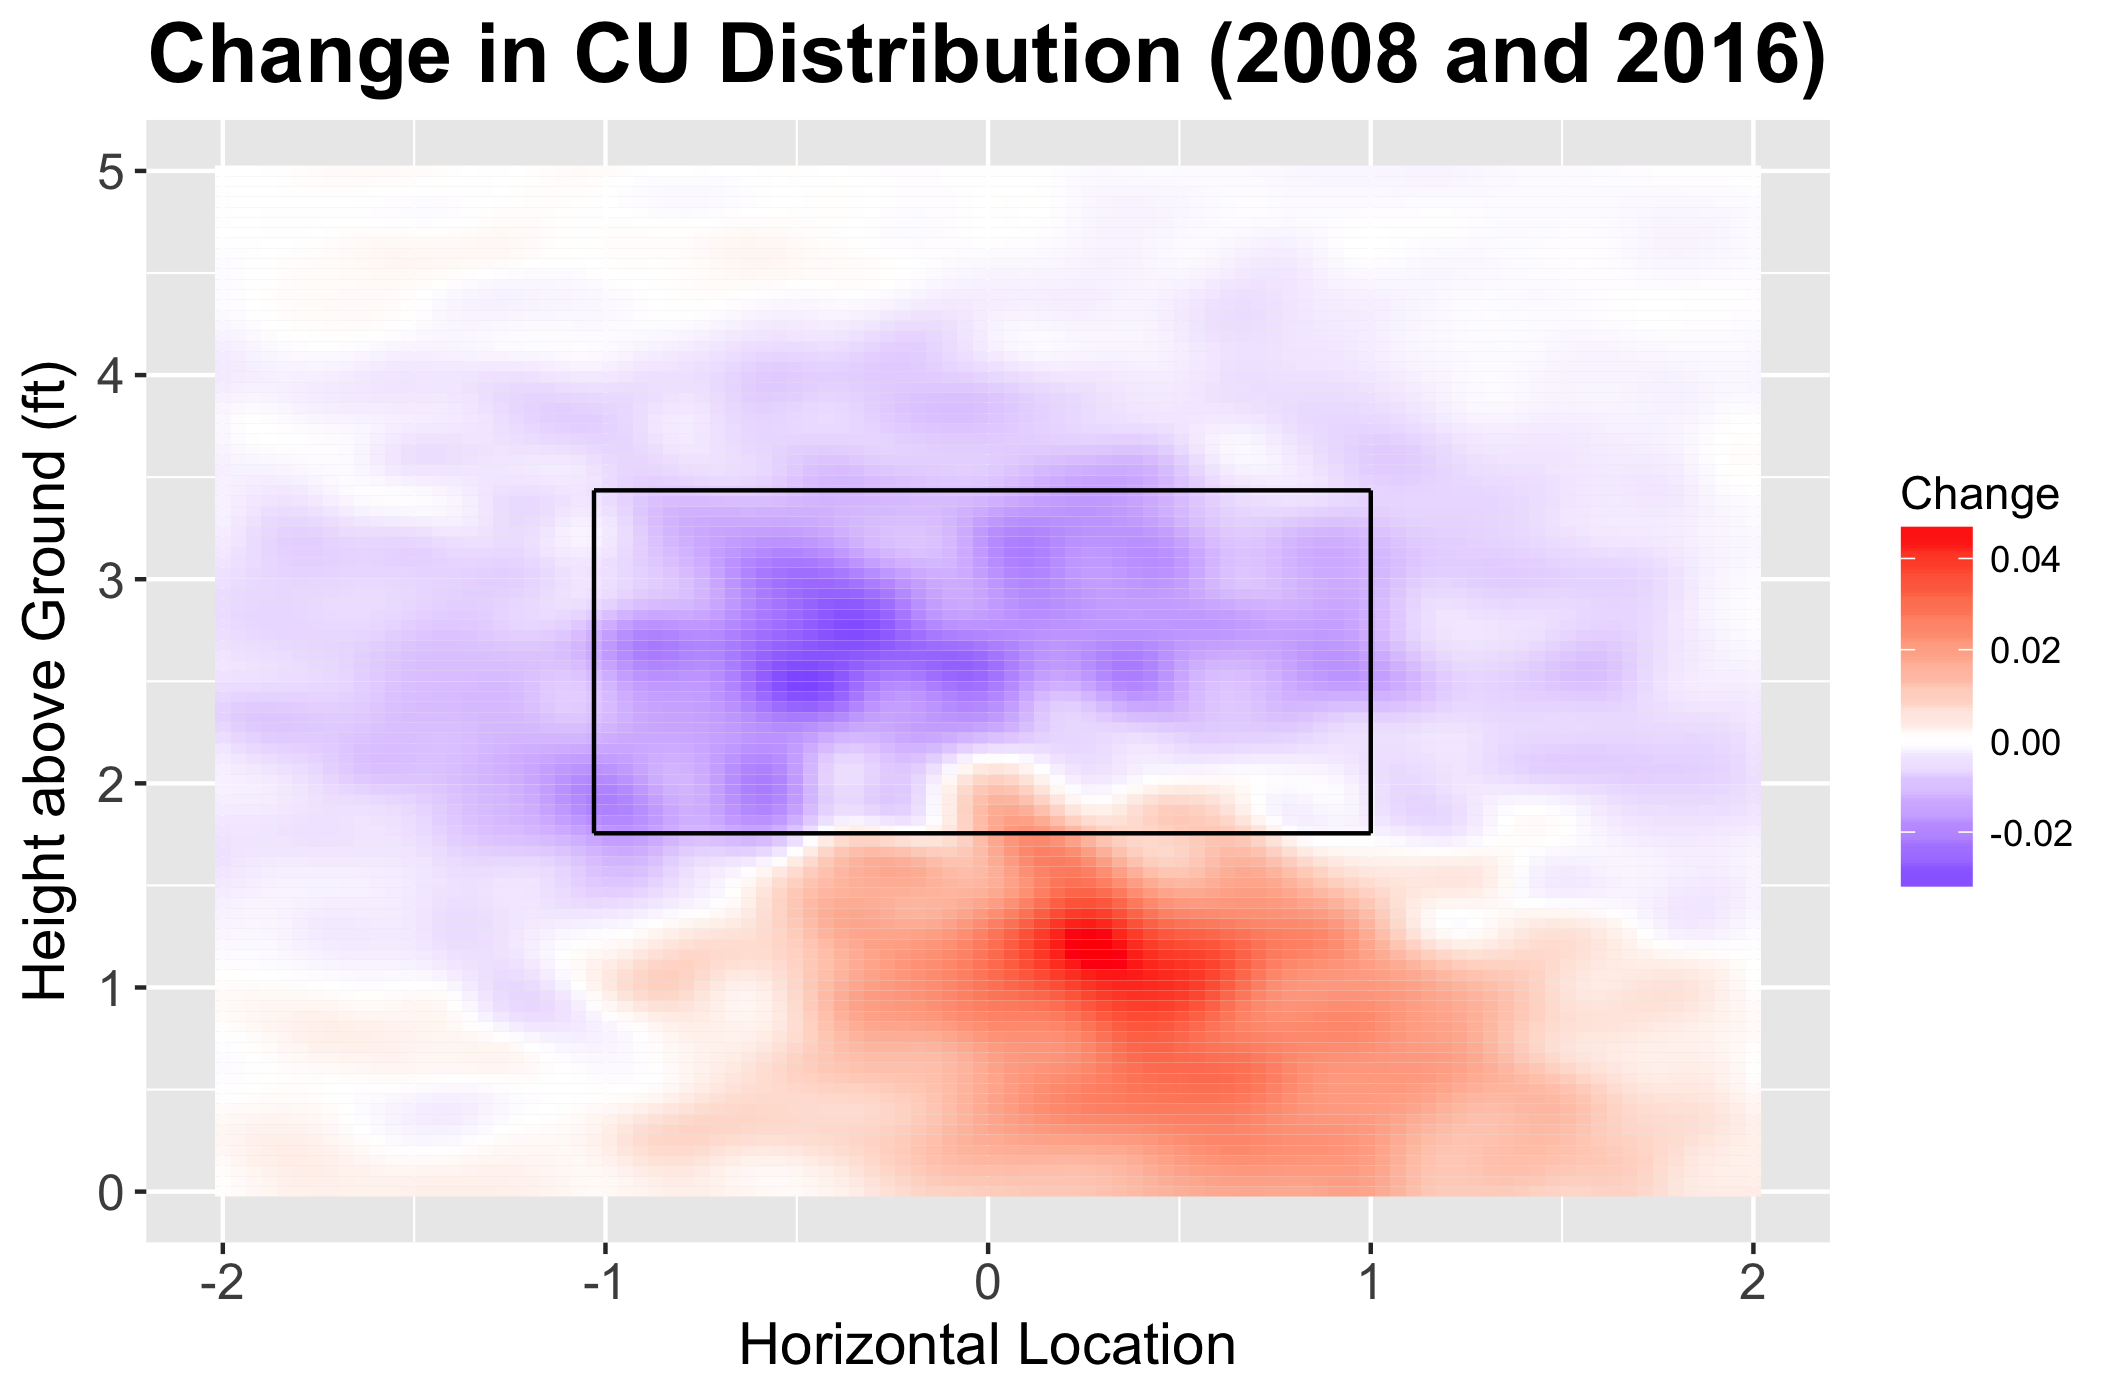
\includegraphics[height = 5.2cm]{../Output/fig3b.png}
\end{subfigure}
\caption{Pitchers Are Throwing Lower Than Ever Before}
\end{figure}

Batters gradually learned that the lower edge of the strike zone was expanding.  As a result, they began swinging at pitches lower in the strike zone with greater frequency.  Interestingly, batters in general were able to discern better between higher pitches outside of the strike zone.  Figure 4a represents the change in model estimates for the probability of a swing on a 3-2 count between 2008 and 2016.  Figure 4b illustrates batter slugging percentage for all balls in play by pitch location during this period of time.

\begin{figure}[ht]
\centering
\begin{subfigure}[b]{0.48\textwidth}
\centering
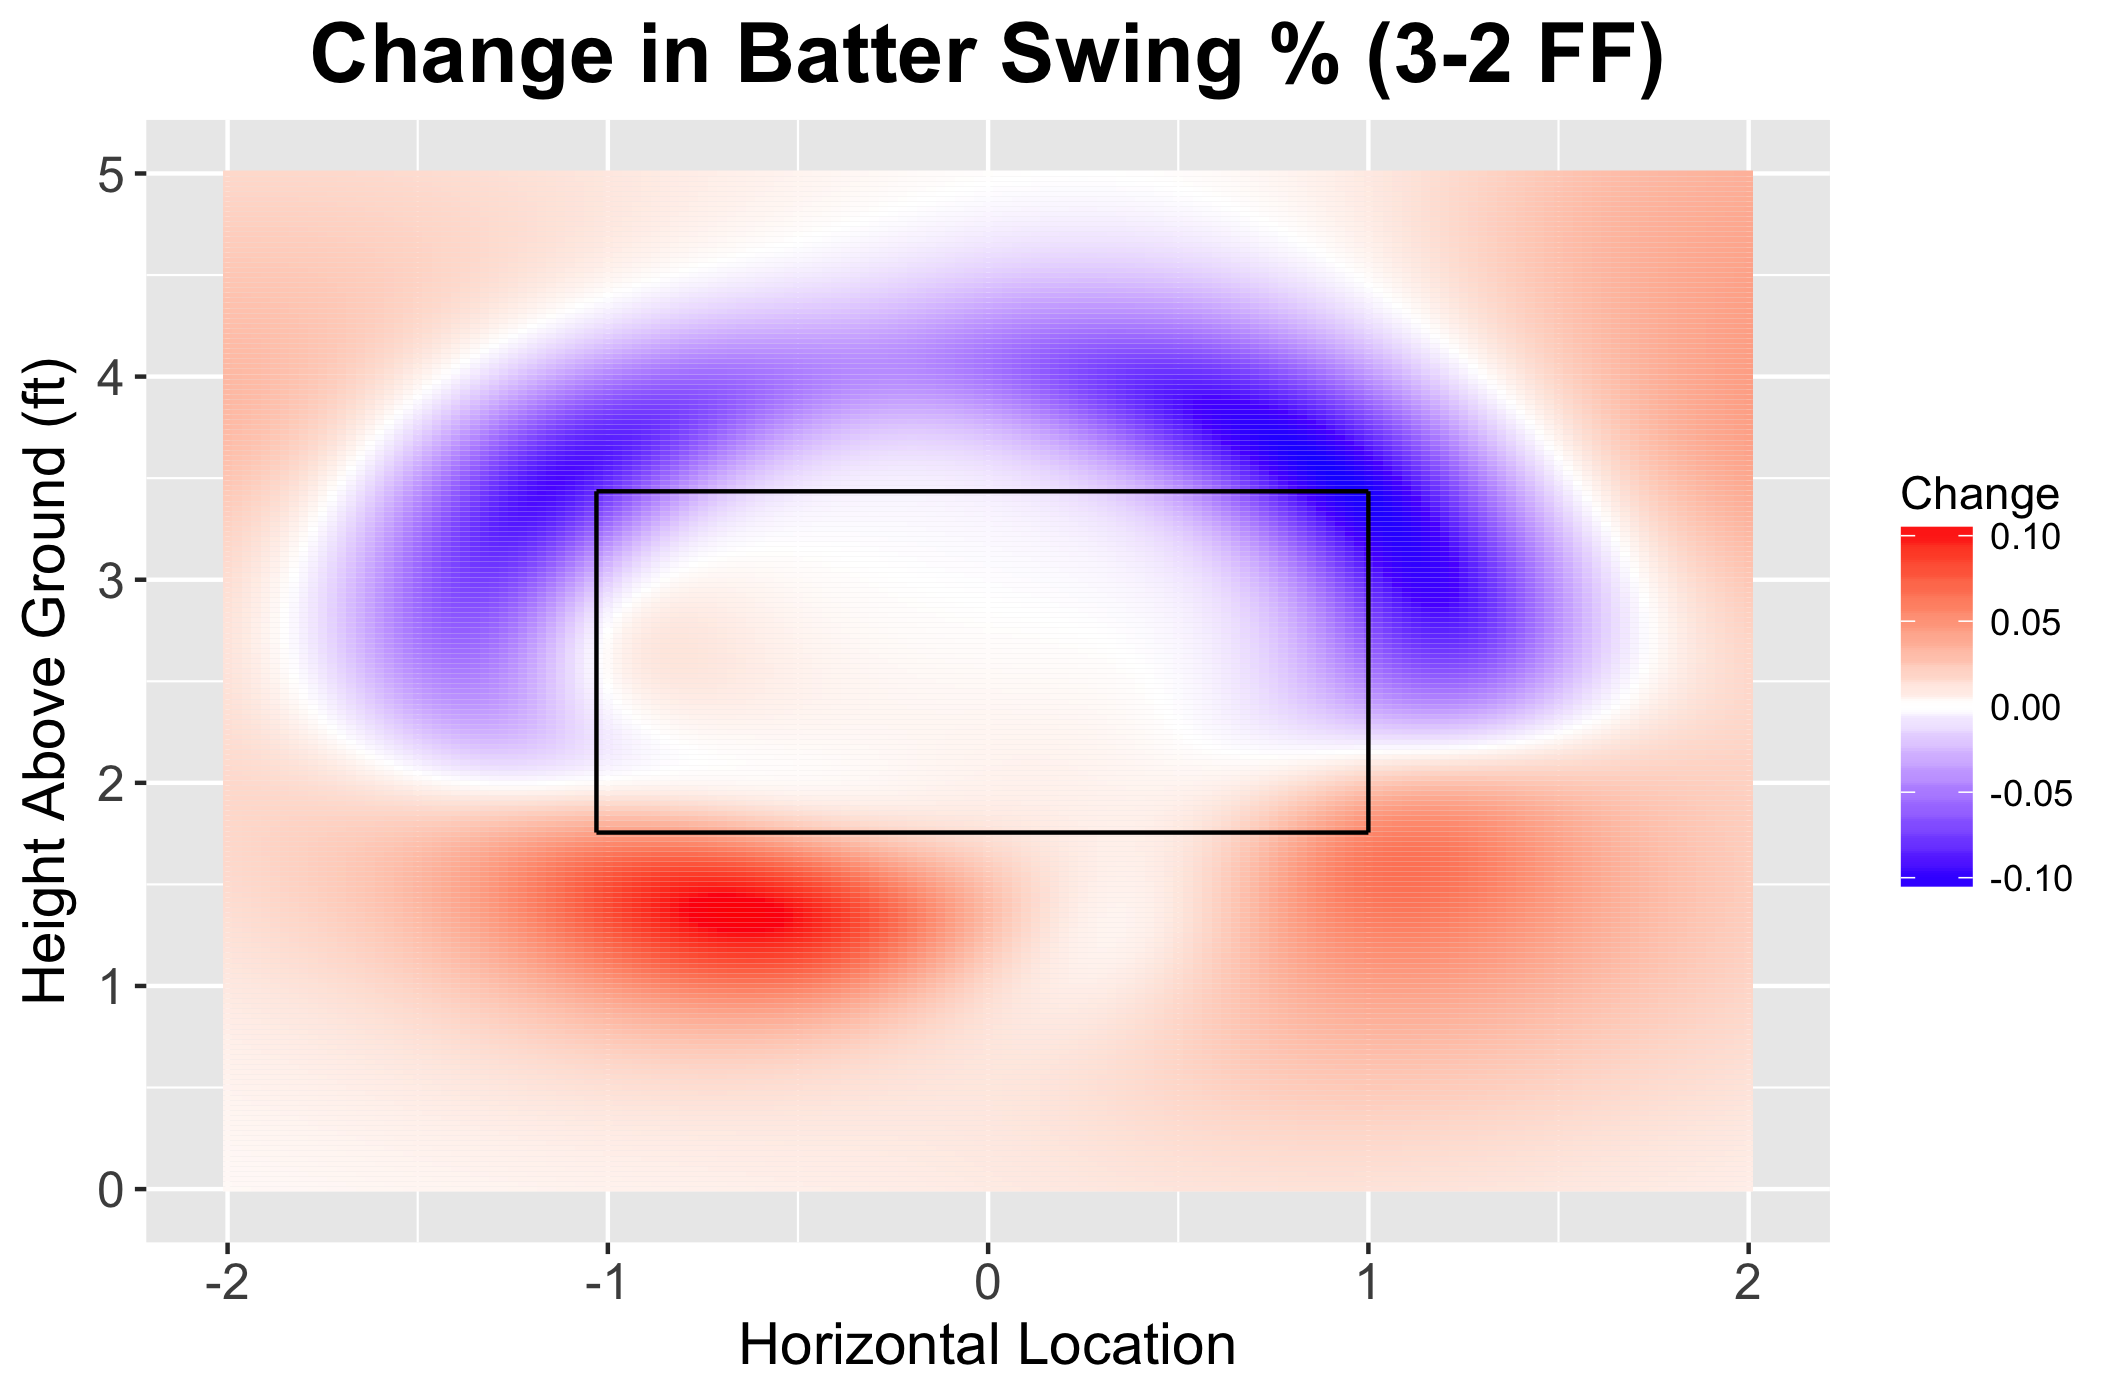
\includegraphics[height = 5.2cm]{../Output/fig4a.png}
\caption{The Evolution of Plate Discipline}
\end{subfigure}
\begin{subfigure}[b]{0.48\textwidth}
\centering
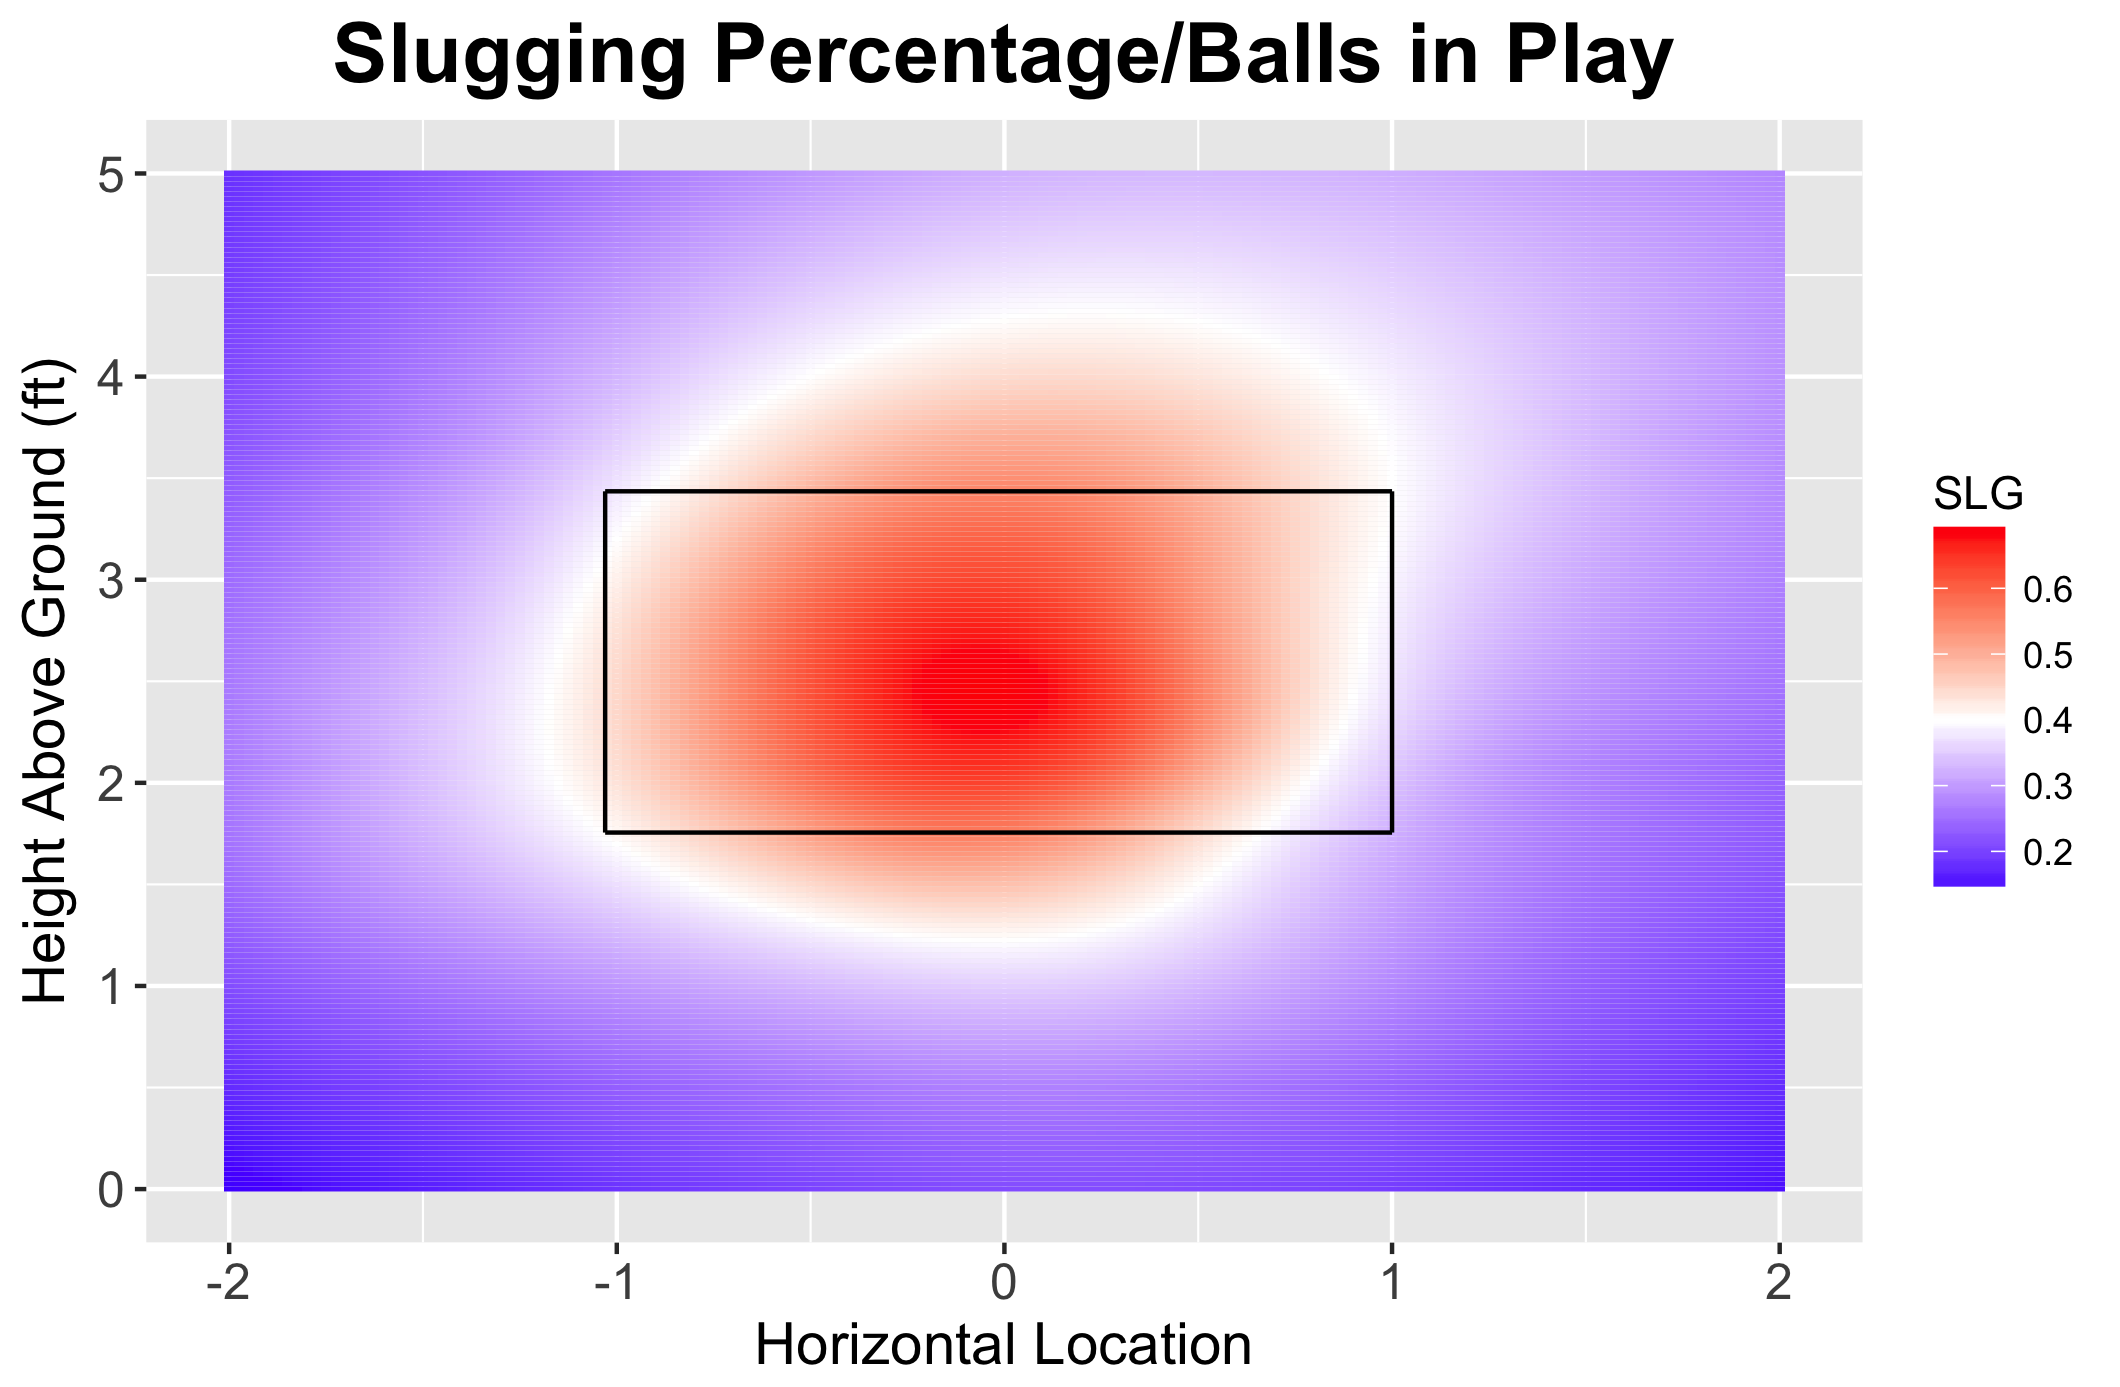
\includegraphics[height = 5.2cm]{../Output/fig4b.png}
\caption{Slugging Percentage by Location}
\end{subfigure}
\caption{Batter Adjustments over Time}
\end{figure}

In sum, both batters and pitchers adjusted to the new rule.  Because batters struggle to hit for power near the lower edge of the zone, pitchers threw lower, enabled by the expanded strike zone.  Batters adjusted by swinging at lower pitches and laying off higher pitches outside of the zone.\\

Will the rule accomplish what the MLB wants?  As illustrated by Figure 5, the overall walk rate has steadily decreased by a total of less than 1\% from 2008 until 2016, when the MLB experienced an uptick in the number of walks.  During that same period, strikeout rates steadily increased by a total of 4\%.  Since teams consistently averaged 38.6 plate appearances per game over this period, we should therefore expect to see an increase of around two ``action plays" per game, assuming these trends are reversed under the new rule.  The MLB should expect to see a slight increase in walks and a sizeable decrease in strikeouts upon implementation.

\begin{figure}[ht]
\centering
\begin{subfigure}[b]{0.48\textwidth}
\centering
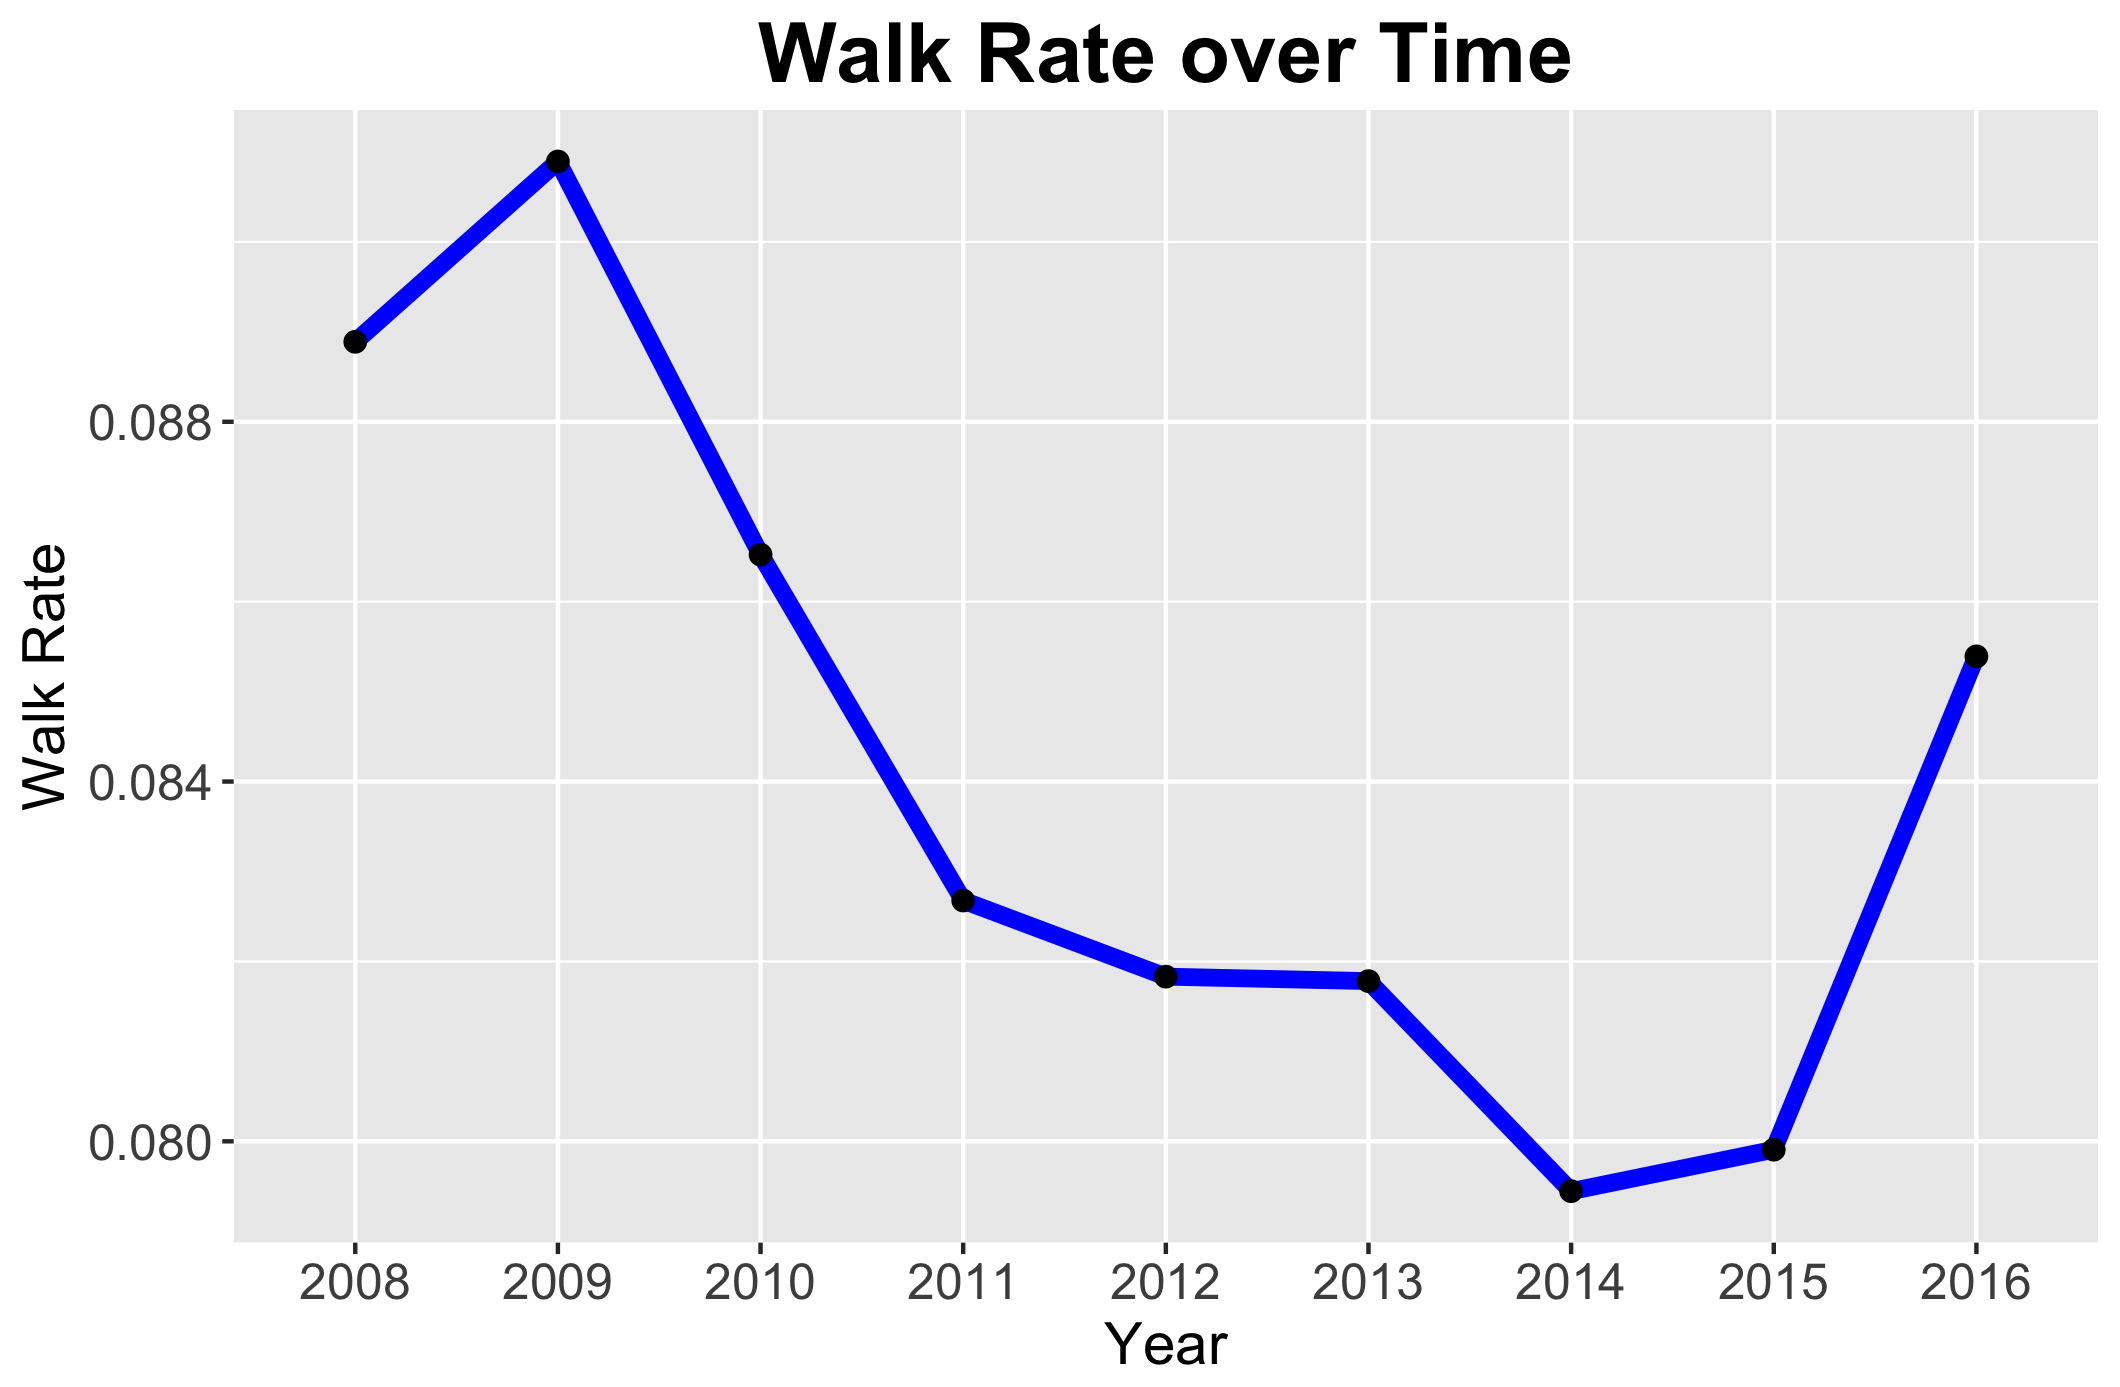
\includegraphics[height = 5.2cm]{../Output/fig5a.png}
\caption{Walk Rate}
\end{subfigure}
\begin{subfigure}[b]{0.48\textwidth}
\centering
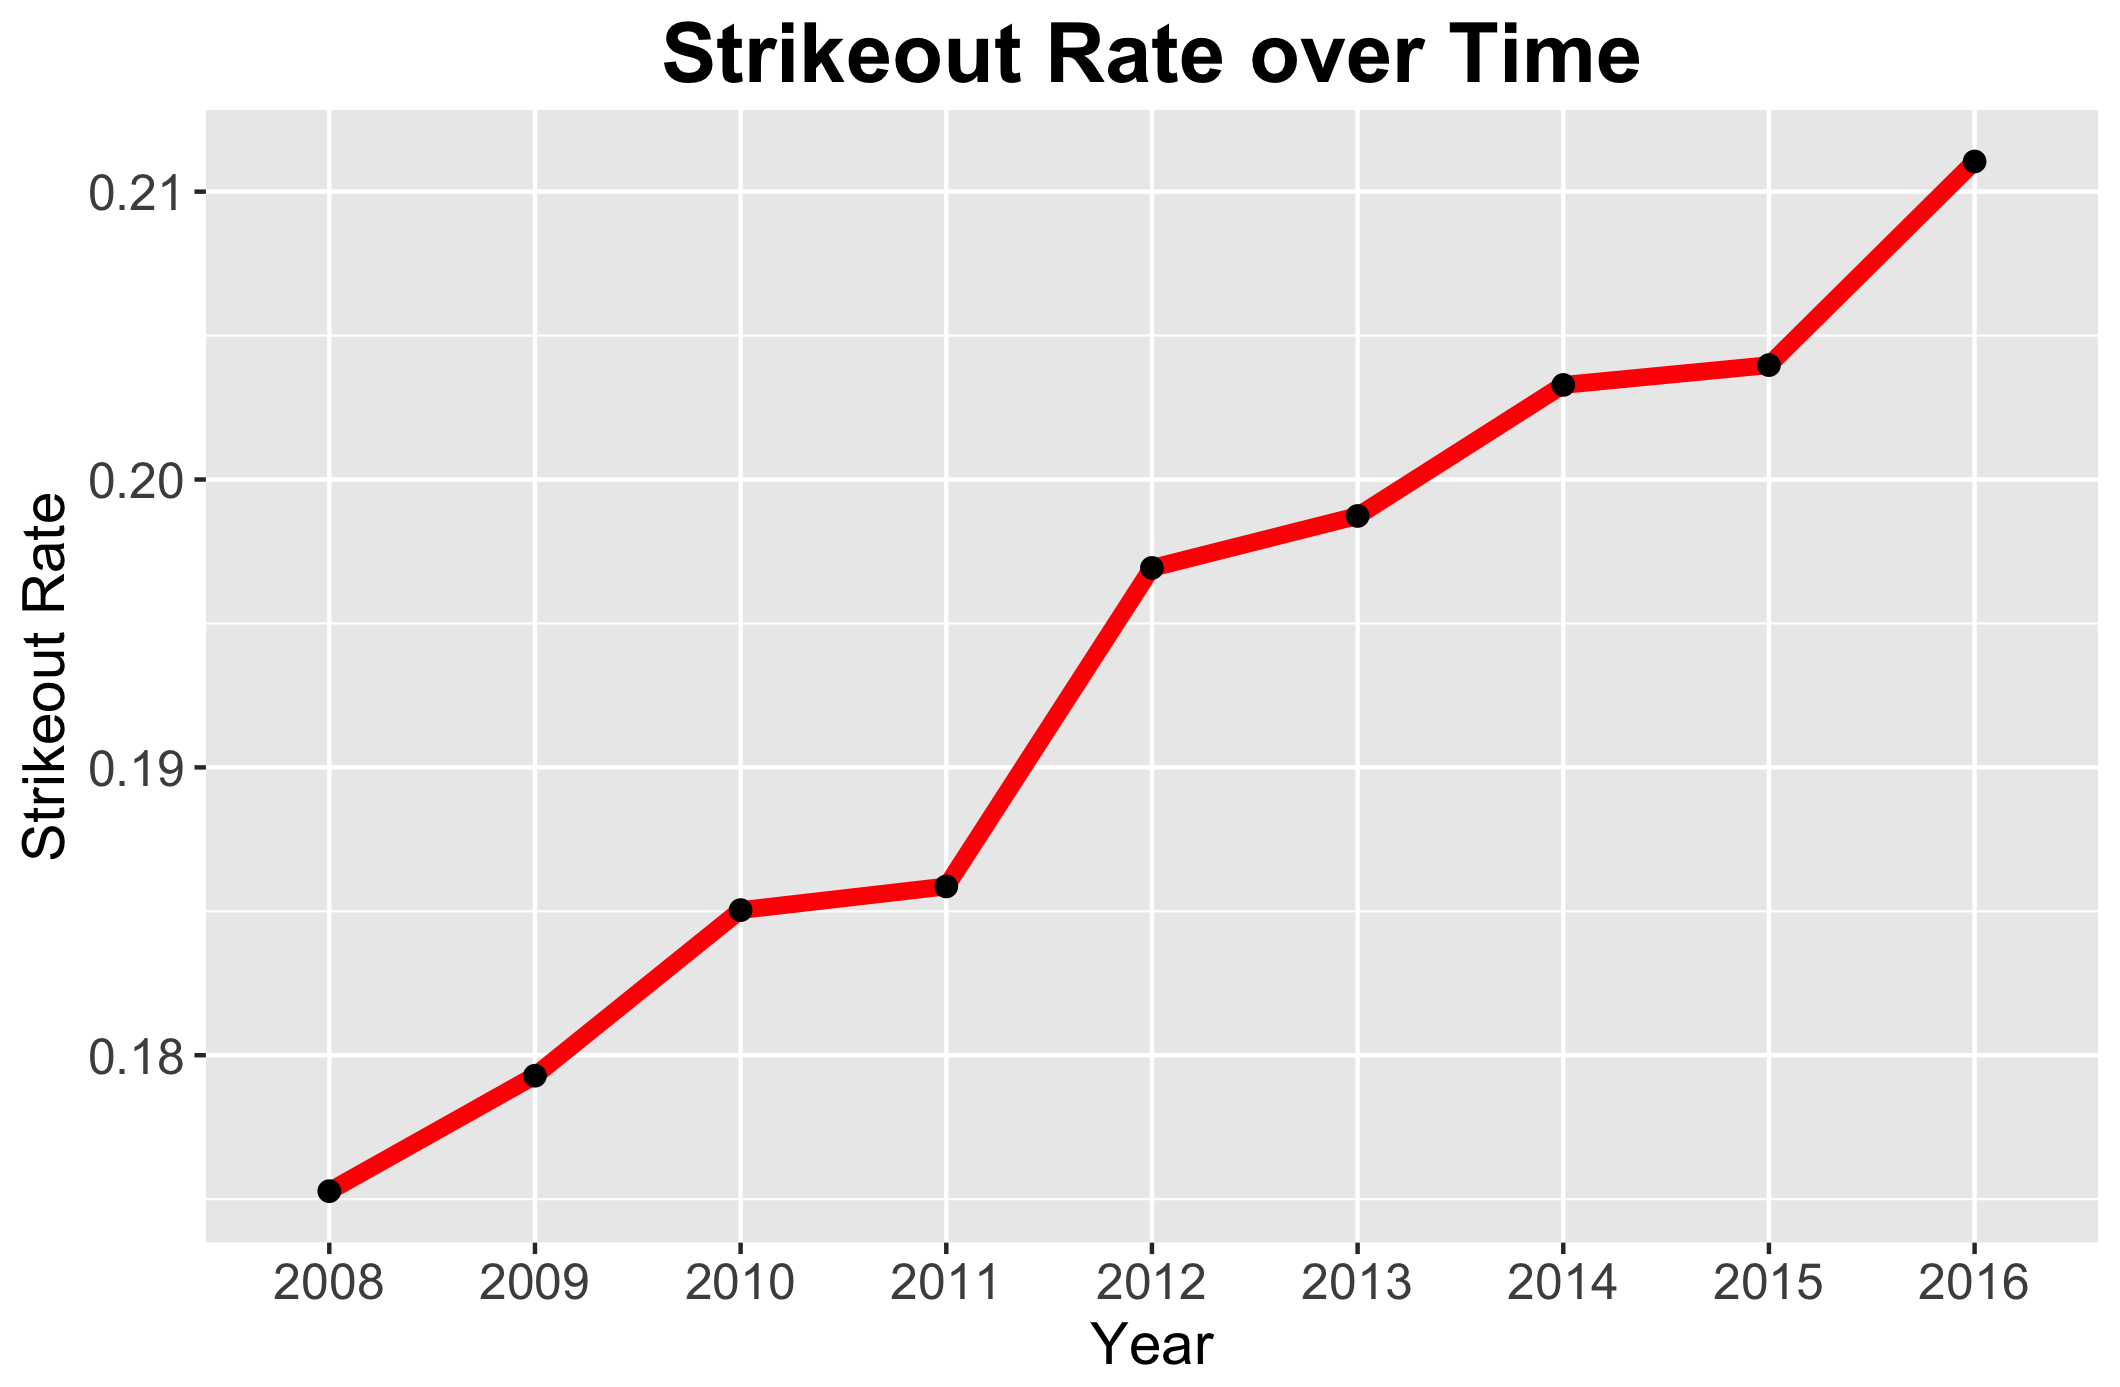
\includegraphics[height = 5.2cm]{../Output/fig5b.png}
\caption{Strikeout Rate}
\end{subfigure}
\caption{Global MLB Changes (2008 - 2016)}
\end{figure}

\section{Individual Impacts: Batters}

\subsection{Measuring Pitch-Level Success - ARG}
Teams try to get every small edge they can with the limited resources that they have.  As such, identifying the players disproportionately helped and/or hurt by raising the strike zone can help teams make profitable decisions at the margin.  To do this, I build upon the work of Joe Sheehan at Baseball Analysts (2008) to calculate the run value of each pitch.  This operates in a similar way to wOBA, but looks at pitch-level data rather than at-bat level data.  For each pitch in 2014 - 2016, I classify the pitch outcome as a ball, strike, hit by pitch, single, double, triple, home run, out, or no change.  All pitches that do not fall within these categories, such as interference, sacrifice bunts, and field errors, are excluded from the analysis.  Table 2 lists the run values of each of these nine outcomes by count.  For example, a strike thrown on a 1-0 count is worth -0.05 runs to the batter and 0.05 runs to the pitcher.  Similarly, a foul ball on a 2-2 count does not change the situation at all, so the pitch run value is neutral to both batter and pitcher.\\  
\newpage

\begin{table}[ht]
\centering
\begin{tabular}{lrrrrrrrrr}
  \hline
Count & Ball & Strike & HBP & Single & Double & Triple & HR & Out & NoC \\ 
  \hline
0-0 & 0.034 & -0.043 & 0.338 & 0.494 & 0.790 & 1.068 & 1.407 & -0.289 & 0.000 \\ 
  1-0 & 0.063 & -0.050 & 0.304 & 0.460 & 0.756 & 1.034 & 1.373 & -0.323 & 0.000 \\ 
  2-0 & 0.110 & -0.062 & 0.241 & 0.397 & 0.693 & 0.971 & 1.310 & -0.385 & 0.000 \\ 
  3-0 & 0.131 & -0.070 & 0.131 & 0.287 & 0.583 & 0.861 & 1.200 & -0.496 & 0.000 \\ 
  0-1 & 0.027 & -0.062 & 0.381 & 0.537 & 0.832 & 1.110 & 1.450 & -0.246 & 0.000 \\ 
  1-1 & 0.050 & -0.067 & 0.354 & 0.510 & 0.805 & 1.083 & 1.423 & -0.273 & 0.000 \\ 
  2-1 & 0.103 & -0.071 & 0.303 & 0.459 & 0.755 & 1.033 & 1.372 & -0.323 & 0.000 \\ 
  3-1 & 0.201 & -0.076 & 0.201 & 0.356 & 0.652 & 0.930 & 1.269 & -0.426 & 0.000 \\ 
  0-2 & 0.022 & -0.184 & 0.442 & 0.598 & 0.894 & 1.172 & 1.511 & -0.184 & 0.000 \\ 
  1-2 & 0.046 & -0.206 & 0.421 & 0.577 & 0.872 & 1.150 & 1.490 & -0.206 & 0.000 \\ 
  2-2 & 0.098 & -0.252 & 0.375 & 0.530 & 0.826 & 1.104 & 1.443 & -0.252 & 0.000 \\ 
  3-2 & 0.276 & -0.351 & 0.276 & 0.432 & 0.728 & 1.006 & 1.345 & -0.350 & 0.000 \\ 
   \hline
\end{tabular}
\caption{Run Values by Pitch Outcome}
\end{table}

By summing the run values of each pitch seen by a batter in a given period, we can calculate the Additional Runs Generated (ARG) for each batter.  To compare batters with differing numbers of at-bats due to injury, we can also calculate the Additional Runs Generated per 100 pitches seen (ARG/100).  Table 3 ranks the top ten and bottom ten batters by ARG from 2014 - 2016.\\

\begin{table}[ht]
\centering
\begin{tabular}{lrr}
  \hline
Batter & ARG & ARG/100 \\ 
  \hline
Mike Trout & 160.535 & 1.754 \\ 
  Paul Goldschmidt & 135.742 & 1.728 \\ 
  Joey Votto & 131.350 & 1.860 \\ 
  Miguel Cabrera & 124.044 & 1.764 \\ 
  Anthony Rizzo & 117.405 & 1.416 \\ 
  Josh Donaldson & 108.238 & 1.229 \\ 
  David Ortiz & 108.183 & 1.466 \\ 
  Bryce Harper & 107.282 & 1.546 \\ 
  Nelson Cruz & 102.407 & 1.285 \\ 
  Freddie Freeman & 97.505 & 1.308 \\ 
   \hline
\end{tabular}
\quad
\begin{tabular}{lrr}
  \hline
Batter & ARG & ARG/100 \\ 
  \hline
Alcides Escobar & -67.906 & -0.918 \\ 
  Omar Infante & -66.602 & -1.551 \\ 
  Billy Hamilton & -58.558 & -1.023 \\ 
  Alexi Amarista & -57.016 & -1.570 \\ 
  Alexei Ramirez & -56.736 & -0.911 \\ 
  Adeiny Hechavarria & -56.545 & -1.020 \\ 
  Ryan Goins & -50.085 & -1.575 \\ 
  Erick Aybar & -49.958 & -0.845 \\ 
  Andrelton Simmons & -48.719 & -0.905 \\ 
  Freddy Galvis & -48.711 & -0.948 \\ 
   \hline
\end{tabular}
\caption{Additional Runs Generated 2014 - 2016 (Batters)}
\end{table}

\subsection{Effect of Zone Change - wRD}

To measure how much each batter would benefit under the new rule, I downweighted pitches that an umpire would be more likely to call a strike in 2016 than in 2008.  Using the generalized additive model discussed earlier to estimate the probability of a called strike, given that the pitch was taken, I define the weight $w_i$ for pitch $i$ to be 
$$ \min(1, 1 + p(\text{Call = Strike} | \text{Taken, Year} = 2008) -  p(\text{Call = Strike} | \text{Taken, Year} = 2016)$$  

From this, I define weighted ARG as follows: $\sum_i (w_i r_i)/ (\sum_i w_i)$, where $r_i$ represents the run value for pitch $i$.  For example, suppose a pitch is located near the lower edge of the strike zone.  The model predicts that this pitch would be a called strike 90\% of the time if taken in 2016, but only 50\% of the time if taken in 2008.  Then the weight of the pitch is $\min(1, 1 + 0.5 - 0.9) = 0.6$.    In essence, this pitch has 60\% of the influence on a batter's weighted ARG that a pitch thrown higher in the zone would have.  Figure 6 illustrates the weights of pitches by strike zone location.  

\begin{figure}[ht]
\centering
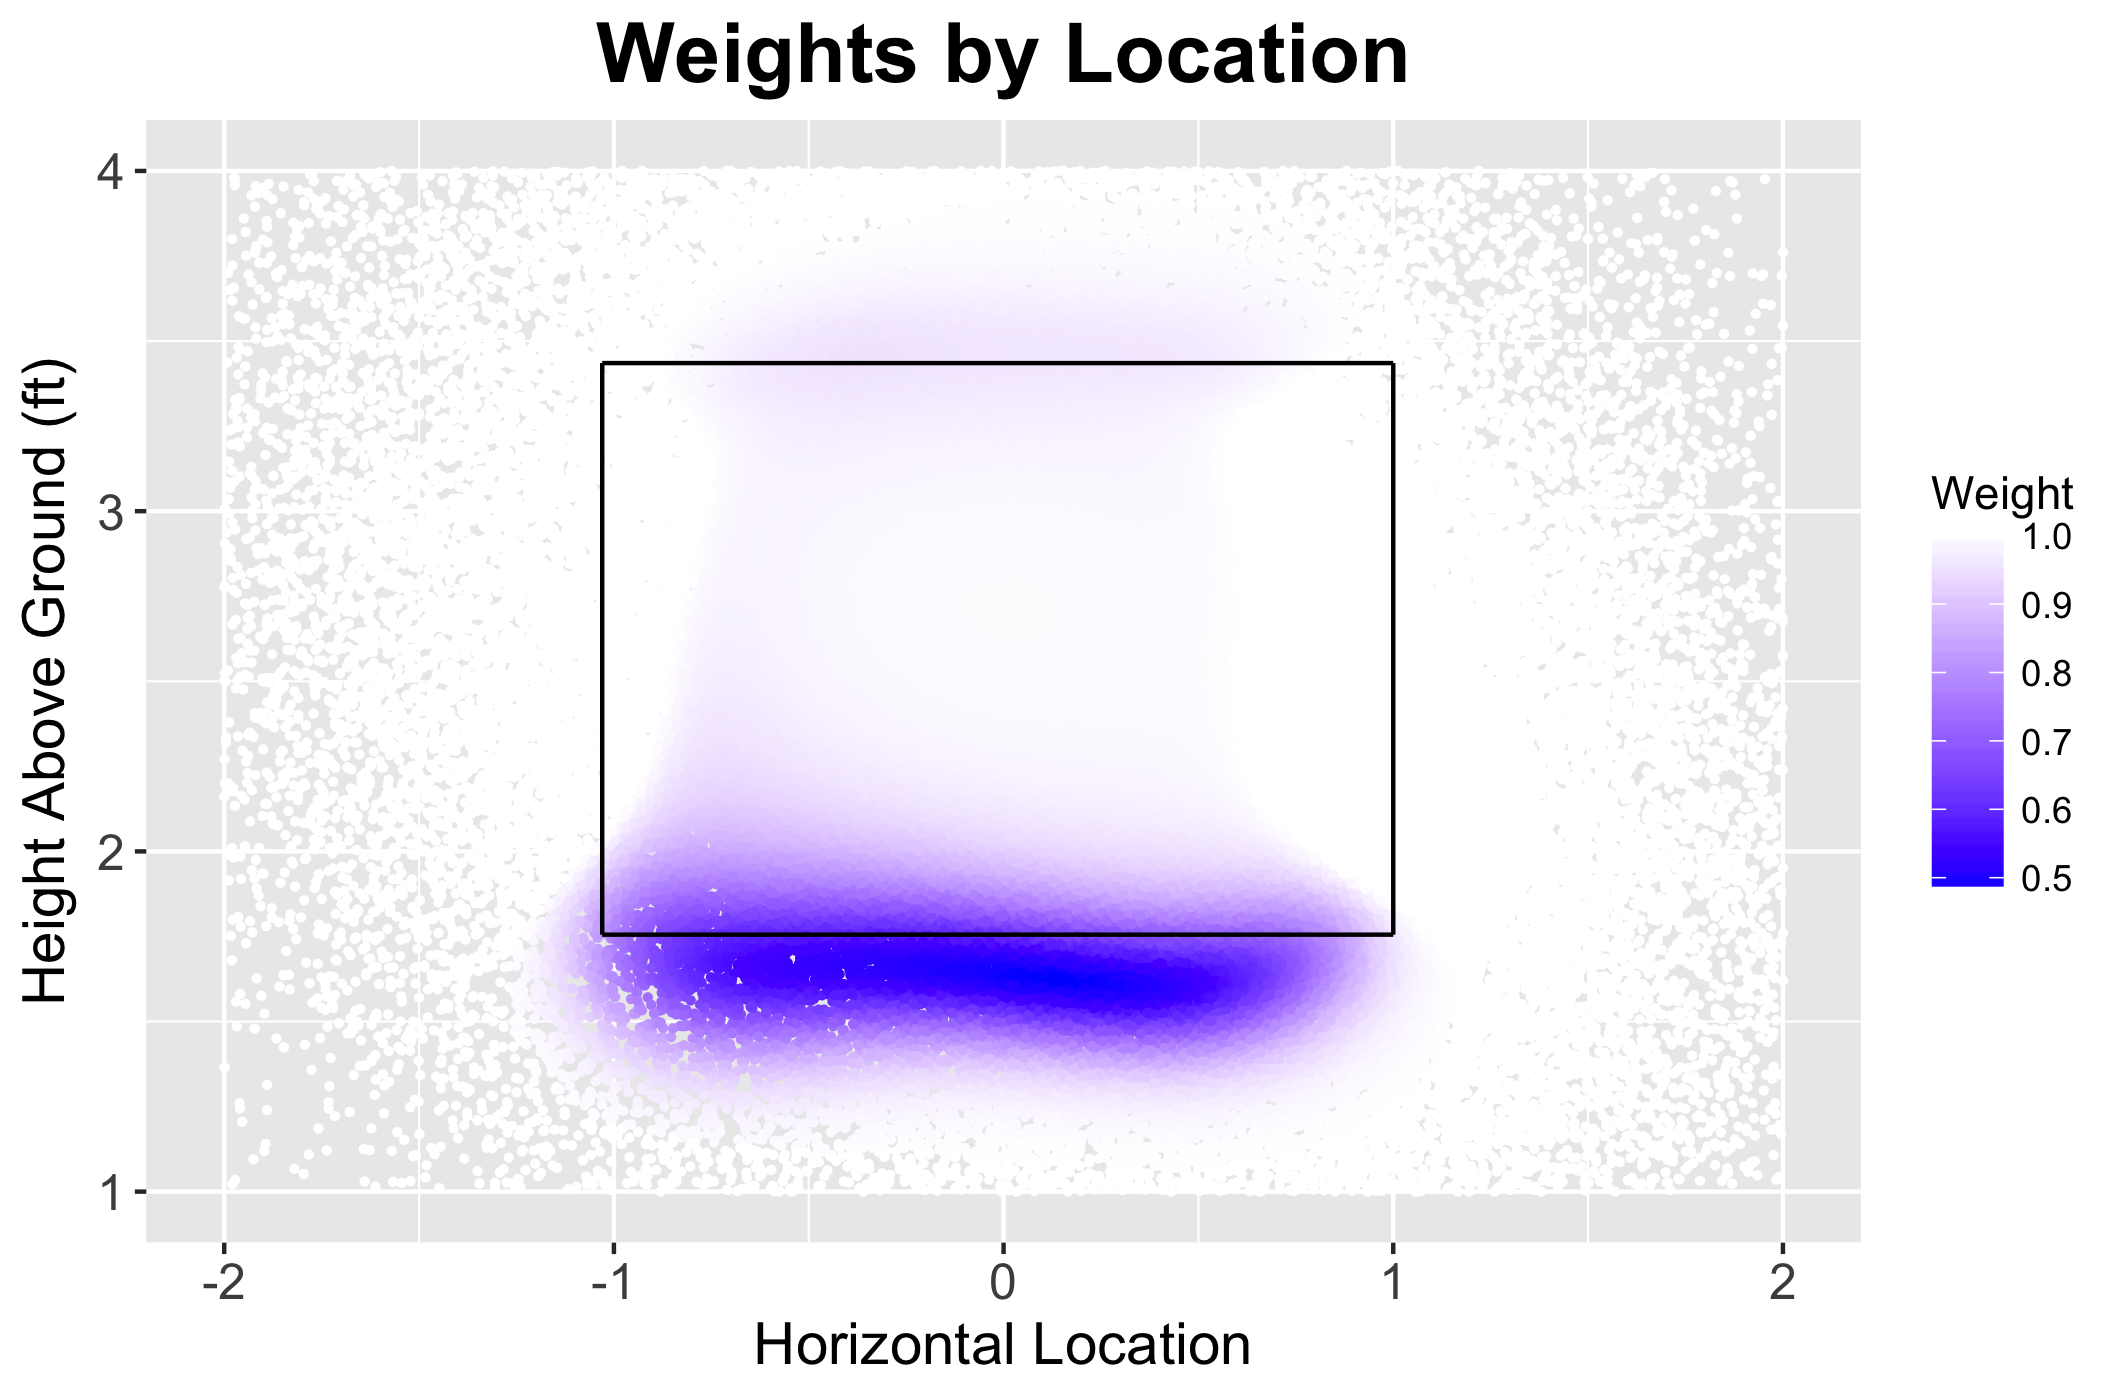
\includegraphics[width = 0.7\textwidth]{../Output/fig6.png}
\caption{Weight Visualization}
\end{figure}

To estimate how many additional runs a batter would generate under the new strike zone, I subtract a batter's ARG from his weighted ARG to obtain a weighted Run Difference (wRD).  The mean seasonal total of weighted Run Difference is within three runs of the actual difference in runs scored in 2008 and runs scored in 2016, a fantastic result.  This means that the weights I used in calculating wRD are almost perfectly calibrated to reflect the changes in scoring between 2008 and 2016.  Table 4 displays the ten highest and lowest wRDs for batters between 2014 and 2016.  Note that the players in the left table struggle to hit low pitches but that the players in the right table are known to be good low ball hitters.

% Fri Feb 17 09:40:49 2017
\begin{table}[ht]
\centering
\begin{tabular}{lr}
  \hline
Batter & WRD \\ 
  \hline
Alex Gordon & 17.561 \\ 
  Christian Yelich & 17.068 \\ 
  Andrew McCutchen & 15.665 \\ 
  Curtis Granderson & 15.041 \\ 
  Carlos Santana & 13.977 \\ 
  Jose Bautista & 13.954 \\ 
  Xander Bogaerts & 13.942 \\ 
  Joe Panik & 13.820 \\ 
  Russell Martin & 13.734 \\ 
  Brett Gardner & 13.244 \\ 
   \hline
\end{tabular}
\quad
\begin{tabular}{lr}
  \hline
Batter & WRD \\ 
  \hline
Chris Parmelee & -3.959 \\ 
  Yoenis Cespedes & -3.149 \\ 
  Mike Trout & -1.967 \\ 
  Tommy Joseph & -1.916 \\ 
  Danny Santana & -1.742 \\ 
  Trevor Story & -1.633 \\ 
  Luis Sardinas & -1.622 \\ 
  Rusney Castillo & -1.491 \\ 
  James McCann & -1.000 \\ 
  Nick Franklin & -0.934 \\ 
   \hline
\end{tabular}
\caption{Weighted Run Difference 2014-2016 (Batters)}
\end{table}

From 2014-2016, I estimate that Alex Gordon would have generated around 17.5 more runs for his team had the new strike zone been in place.  While we should expect some regression to the mean going forward, this difference is no fluke.  Between 2014 and 2016, the year to year correlation in wRD was 0.32.  When expanded to use the sum of 2014 and 2015 wRD to predict 2016, the correlation rose to 0.47, roughly equivalent to the year to year correlation of batting average and slightly below that of wOBA. This implies that we can project these values to future seasons with some degree of confidence; Alex Gordon will continue to comparatively struggle hitting low pitches and Mike Trout will continue rocking balls on the lower edge.\\

The actionable intelligence here is simple: players with high wRD values will benefit more from the rule to raise the lower edge of the strike zone than players with low wRD values.  The question then arises: how much more money should the market be willing to pay players with high wRD values such as Alex Gordon?  Batter wRD is usually positive, since most players struggle to hit low pitches as well as they hit other pitches, which results in run inflation.  To account for this, I adjust wRD by substracting overall mean wRD per pitch and multiply by the total number of pitches seen by a batter.  In other words, adjusted wRD tells us how many additional runs a batter would produce under the new rule above and beyond the improvement expected of him if he improved at an average rate.  Table 5 depicts the top ten and bottom ten players in terms of adjusted wRD.

\begin{table}[ht]
\centering
\begin{tabular}{lr}
  \hline
Batter & wRD \\ 
  \hline
Alex Gordon & 9.349 \\ 
  Christian Yelich & 8.093 \\ 
  Joe Panik & 7.948 \\ 
  Matt Joyce & 6.872 \\ 
  Stephen Vogt & 6.673 \\ 
  Andrew McCutchen & 6.068 \\ 
  Chris Coghlan & 6.067 \\ 
  Russell Martin & 5.953 \\ 
  Shin-Soo Choo & 5.804 \\ 
  Jason Castro & 5.740 \\ 
   \hline
\end{tabular}
\quad
\begin{tabular}{lr}
  \hline
Batter & wRD \\ 
  \hline
Mike Trout & -12.735 \\ 
  Yoenis Cespedes & -11.991 \\ 
  Adam Jones & -8.168 \\ 
  Brandon Belt & -7.399 \\ 
  Yadier Molina & -7.041 \\ 
  Carlos Gonzalez & -7.027 \\ 
  Eduardo Escobar & -6.587 \\ 
  Eugenio Suarez & -6.521 \\ 
  Denard Span & -6.328 \\ 
  Matt Kemp & -6.052 \\ 
   \hline
\end{tabular}
\caption{Adjusted wRD 2014 - 2016 (Batters)}
\end{table}

Assuming a conservative 50\% regression toward the mean, roughly 9 runs/WAR, and a market value of \$8 million per WAR, I estimate that Alex Gordon is worth around \$1.3 million more per year when the new rule is implemented.  Conversely, I estimate that Mike Trout will be worth around \$2 million less per year once the strike zone is raised.  While these numbers aren't enormous, they aren't negligible either.  Knowing a player's adjusted wRD can save teams a few million dollars per year, assuming that not all teams price wRD into their player valuation framework. 

\section{Individual Impact: Pitchers}
The same approach that we used for batters can also be used for pitchers.  I define and calculate ARG, ARG/100, wRD and adjusted wRD the exact same way as before.  The only difference is that negative wRD and ARG values are good for pitchers, since these metrics now correspond to additional runs allowed.  Table 6 presents the top ten pitchers in the MLB in terms of ARG (left) and ARG/100 (right) between 2014 and 2016.\\

\begin{table}[ht]
\centering
\begin{tabular}{lrr}
  \hline
Pitcher & ARG & ARG/100 \\ 
  \hline
Clayton Kershaw & -199.774 & -2.258 \\ 
  Jake Arrieta & -167.744 & -1.744 \\ 
  Madison Bumgarner & -140.265 & -1.265 \\ 
  Johnny Cueto & -123.531 & -1.160 \\ 
  Max Scherzer & -121.746 & -1.128 \\ 
  Corey Kluber & -118.278 & -1.134 \\ 
  Jon Lester & -112.492 & -1.059 \\ 
  Chris Sale & -106.136 & -1.122 \\ 
  Zack Greinke & -103.928 & -1.139 \\ 
  David Price & -95.466 & -0.854 \\ 
   \hline
\end{tabular}
\quad
\begin{tabular}{lrr}
  \hline
Pitcher & ARG & ARG/100\\ 
  \hline
Andrew Miller & -83.360 & -2.409 \\ 
  Mark Melancon & -74.082 & -2.353 \\ 
  Wade Davis & -77.912 & -2.345 \\ 
  Clayton Kershaw & -199.774 & -2.258 \\ 
  Zach Britton & -67.367 & -2.204 \\ 
  Kenley Jansen & -62.283 & -2.018 \\ 
  Aroldis Chapman & -64.734 & -1.949 \\ 
  Seung Hwan Oh & -25.063 & -1.934 \\ 
  Dellin Betances & -76.381 & -1.921 \\ 
  Carson Smith & -22.762 & -1.866 \\ 
   \hline
\end{tabular}
\caption{Adjusted Runs Generated 2014 - 2016 (Pitchers)}
\end{table}

\newpage 
Interestingly, the top pitchers in terms of ARG are premier starters in the league, while the top pitchers in terms of ARG/100 are strong relievers, with the notable exception of Clayton Kershaw.  This means that the top starters are more productive, but the top relievers are more efficient, an observation consistent with baseball intuition.  Table 7 presents the top 10 highest and lowest adjusted wRD values for pitchers over the period studied.

\begin{table}[ht]
\centering
\begin{tabular}{lrr}
  \hline
Pitcher & wRD & Adj wRD \\ 
  \hline
Felix Hernandez & 21.863 & 11.393 \\ 
  Sonny Gray & 18.795 & 9.045 \\ 
  Tim Hudson & 14.780 & 9.008 \\ 
  Kyle Gibson & 17.585 & 7.647 \\ 
  Martin Perez & 13.125 & 7.098 \\ 
  Francisco Liriano & 16.003 & 6.072 \\ 
  Masahiro Tanaka & 14.568 & 5.998 \\ 
  Scott Kazmir & 15.473 & 5.613 \\ 
  Jake Arrieta & 16.909 & 5.590 \\ 
  Dallas Keuchel & 16.604 & 5.584 \\ 
   \hline
\end{tabular}
\quad
\begin{tabular}{lrr}
  \hline
Pitcher & wRD & Adj wRD\\ 
  \hline
David Price & 4.487 & -8.669 \\ 
  Dan Haren & -0.770 & -7.791 \\ 
  Chris Tillman & 3.729 & -7.474 \\ 
  Justin Verlander & 3.530 & -7.414 \\ 
  Drew Smyly & 0.553 & -7.211 \\ 
  Max Scherzer & 6.080 & -6.618 \\ 
  Chris Sale & 4.705 & -6.429 \\ 
  Jose Quintana & 5.377 & -6.342 \\ 
  Chris Archer & 6.390 & -5.346 \\ 
  Matt Wisler & -0.067 & -4.999 \\ 
   \hline
\end{tabular}
\caption{Adjusted wRD 2014 - 2016 (Pitchers)}
\end{table}

Suprisingly, wRD is even slightly more robust for pitchers than it is for batters.  The year to year correlation in wRD is 0.38, placing it squarely between hallmarks such as ERA and FIP.  This correlation increases to 0.45 when predicting 2016 wRD from both 2014 and 2015 data.  Hence, while we should expect some regression to the mean in future seasons, pitchers with high wRDs will also tend to have high wRDs in the future.\\

The pitchers who will suffer the most are those that rely on low, sinking pitches to induce ground balls.  Chief among these is King Felix Hernandez.  If the rule is implemented next season, he should see his value drop in the neighborhood of \$1.9 million per year over the next few seasons, making the same assumptions as were made for batters.  On the other hand, pitchers such as David Price and Dan Haren do not rely heavily on the lower edge of the zone to get batters out, so they will see their estimated value increase by around \$1.2 million per year over the next few seasons.  

\section{Future Work: Catcher Framing and MiLB Players}
In this analysis, I examined the effect of raising the bottom edge of the strike zone by two inches for both MLB batters and pitchers.  Batters and pitchers will not be the only players affected by this new rule, however.  As the strike zone shrinks, catcher framing of low pitches will become more important, particularly in the first season as umpires adjust to the new rule.  Finding which catchers are better at framing low pitches and projecting that onto the new strike zone is a very worthwhile problem, but one I did not have time to explore in the two week window.   A similar method of comparing catcher framing in 2008 and 2016 could be one possible path, though there are many confounders involved.\\

Teams could reap the largest return from this research by using it to project minor league performance under the new strike zone.  If prospects struggle hitting low pitches, they may benefit disproportionately under the new rule.  Identifying those players can help general managers make more advantageous trades for prospects and selections in the Rule 5 draft.

\section{Appendix - Introduction to Smoothing Splines}
In this analysis, to model the probability of a strike at a given pitch location, I fit a thin-plate logistic regression smoothing spline.  To avoid detracting from the findings while still giving the reader necessary background on what I'm doing, I present a brief overview of smoothing splines here.\\

\subsection{Univariate Splines}
In the one-dimensional case, we assume that the dependent variable $y$ is a noisy function of an independent variable $x$.  We observe a total of $n$ $(x_i, y_i)$ coordinate pairs.  If this relationship is linear, we can model the relationship by a linear regression if $y$ takes on continuous values or logistic regression if $y$ takes on binary values.  Sometimes, the relationship between $y$ and $x$ is highly non-linear and it's unclear what the mathematical relationship between the two of them is.  In that case, fitting a smoothing spline is a principled way to find a function that fits the data well.\\

Mathematically, we seek to find a twice-differentiable function $\hat{f}(x)$ that minimizes the following expression:

\begin{equation}
\sum_{i = 1}^n (y_i - \hat{f}(x_i))^2) + \lambda \int_{x_1}^{x_n} \hat{f}^{''}(x)^2 dx
\end{equation}

where $\hat{f}''$ is the second derivative of $\hat{f}$ and $\lambda$ is a tuning parameter that penalizes extreme values of the derivative of $\hat{f}$.  If $\lambda = 0$, the smoothing spline is equivalent to drawing a line graph between consecutive points.  As the penalty parameter $\lambda$ increases, the function $\hat{f}$ becomes more smooth.  Figure 7 illustrates a simple smoothing spline fit under different values of $\lambda$.  Note that the red dashed line corresponds to a higher value of $\lambda$.\\

\begin{figure}[ht]
\centering
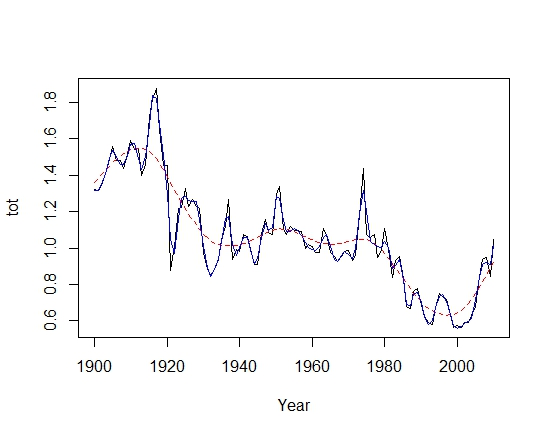
\includegraphics[width = 0.7\textwidth]{../Output/fig7.jpg}
\caption{A Simple Smoothing Spline}
\end{figure}

How do we choose $\lambda$?  We choose it through a process called cross-validation, in which some of the data is held out.  For each value of $\lambda$, we find the optimal function $\hat{f}$ under the remaining data and see how well we predict the held out data.  We do this ten times, holding out each observation exactly once, and choose the value of $\lambda$ that results in the best out-of-sample predictions. \\

\subsection{Modeling the Strike Zone with Splines}
Modeling the strike zone based on location and umpire decisions with a smoothing spline takes the same ideas and generalizes them to two-dimensions and a binary dependent variable.  The expression to minimize is now equal to the following:

\begin{equation}
\sum_{i = 1}^n (-y_i \hat{f}(x,z) + \log(1 + e^{\hat{f}(x,z)})) + \lambda \int_{x_1}^{x_n} \int_{z_1}^{z_n}\frac{\partial\hat{f}}{\partial x}^2 + 2 \frac{\partial\hat{f}}{\partial x}\frac{\partial\hat{f}}{\partial z} + \frac{\partial\hat{f}}{\partial z}^2dz dx
\end{equation}    

Computationally, we can estimate this using the \texttt{mgcv} package in R,  a wonderful resource for fitting generalized additive models.  Once we find $\hat{f}$, we can predict the probability that $y = 1$ to data that we have not even seen before.  The difference in predictions from $\hat{f}$ fit with the 2008 data and $\hat{f}$ fit with the 2016 data forms the backbone behind the metric wRD defined in the analysis. 
\newpage 
\section{References}
\begin{itemize}
\item Mike Fast (2011).  \textit{Spinning Yarn - A Zone of their Own}.  \\
http://www.baseballprospectus.com/article.php/articleid=14572  
\item Brian Grosnick (2014). \textit{Converting Runs to Wins in 2013}.\\ http://www.beyondtheboxscore.com/2014/4/10/5591522/converting-runs-to-wins-in-2013-wins-above-replacement-sabermetrics-ugh-math
\item David Leonhardt (2014). \textit{The Strike Zone Revolution}.  The New York Times.\\
https://www.nytimes.com/2014/10/24/upshot/the-strike-zone-revolution.html
\item Bill Petti (2011). \textit{What Hitting Metrics Correlate Year to Year}.\\
http://www.beyondtheboxscore.com/2011/9/1/2393318/what-hitting-metrics-are-consistent-year-to-year
\item Bill Petti (2012). \textit{What Starting Pitcher Metrics Correlate Year to Year}.\\
http://www.beyondtheboxscore.com/2012/1/9/2690405/what-starting-pitcher-metrics-correlate-year-to-year
\item Joe Sheehan (2008).  \textit{More Run Values}.\\
http://baseballanalysts.com/archives/2008/02/writing\_about\_t.php
\item Carson Sievert (2015). pitchRx: Tools for Harnessing 'MLBAM' 'Gameday' Data and Visualizing 'pitchfx'. R package version 1.8.2.
\item Jayson Stark (2017). \textit{MLB proposes changes to intentional walk, strike zone}.  ESPN.\\
http://www.espn.com/mlb/story/\_/id/18631714/mlb-proposes-scrapping-intentional-walk-raising-strike-zone
\item Neil Weinberg (2016). \textit{Basic Principles of Free Agent Contract Negotiation}.\\
http://www.fangraphs.com/library/basic-principles-of-free-agent-contract-evaluation/

\end{itemize}



    
\end{document}